\documentclass[mstat,12pt]{unswthesis}

\usepackage{color}
\usepackage{fancyvrb}
\newcommand{\VerbBar}{|}
\newcommand{\VERB}{\Verb[commandchars=\\\{\}]}
\DefineVerbatimEnvironment{Highlighting}{Verbatim}{commandchars=\\\{\}}
% Add ',fontsize=\small' for more characters per line
\usepackage{framed}
\definecolor{shadecolor}{RGB}{248,248,248}
\newenvironment{Shaded}{\begin{snugshade}}{\end{snugshade}}
\newcommand{\AlertTok}[1]{\textcolor[rgb]{0.94,0.16,0.16}{#1}}
\newcommand{\AnnotationTok}[1]{\textcolor[rgb]{0.56,0.35,0.01}{\textbf{\textit{#1}}}}
\newcommand{\AttributeTok}[1]{\textcolor[rgb]{0.77,0.63,0.00}{#1}}
\newcommand{\BaseNTok}[1]{\textcolor[rgb]{0.00,0.00,0.81}{#1}}
\newcommand{\BuiltInTok}[1]{#1}
\newcommand{\CharTok}[1]{\textcolor[rgb]{0.31,0.60,0.02}{#1}}
\newcommand{\CommentTok}[1]{\textcolor[rgb]{0.56,0.35,0.01}{\textit{#1}}}
\newcommand{\CommentVarTok}[1]{\textcolor[rgb]{0.56,0.35,0.01}{\textbf{\textit{#1}}}}
\newcommand{\ConstantTok}[1]{\textcolor[rgb]{0.00,0.00,0.00}{#1}}
\newcommand{\ControlFlowTok}[1]{\textcolor[rgb]{0.13,0.29,0.53}{\textbf{#1}}}
\newcommand{\DataTypeTok}[1]{\textcolor[rgb]{0.13,0.29,0.53}{#1}}
\newcommand{\DecValTok}[1]{\textcolor[rgb]{0.00,0.00,0.81}{#1}}
\newcommand{\DocumentationTok}[1]{\textcolor[rgb]{0.56,0.35,0.01}{\textbf{\textit{#1}}}}
\newcommand{\ErrorTok}[1]{\textcolor[rgb]{0.64,0.00,0.00}{\textbf{#1}}}
\newcommand{\ExtensionTok}[1]{#1}
\newcommand{\FloatTok}[1]{\textcolor[rgb]{0.00,0.00,0.81}{#1}}
\newcommand{\FunctionTok}[1]{\textcolor[rgb]{0.00,0.00,0.00}{#1}}
\newcommand{\ImportTok}[1]{#1}
\newcommand{\InformationTok}[1]{\textcolor[rgb]{0.56,0.35,0.01}{\textbf{\textit{#1}}}}
\newcommand{\KeywordTok}[1]{\textcolor[rgb]{0.13,0.29,0.53}{\textbf{#1}}}
\newcommand{\NormalTok}[1]{#1}
\newcommand{\OperatorTok}[1]{\textcolor[rgb]{0.81,0.36,0.00}{\textbf{#1}}}
\newcommand{\OtherTok}[1]{\textcolor[rgb]{0.56,0.35,0.01}{#1}}
\newcommand{\PreprocessorTok}[1]{\textcolor[rgb]{0.56,0.35,0.01}{\textit{#1}}}
\newcommand{\RegionMarkerTok}[1]{#1}
\newcommand{\SpecialCharTok}[1]{\textcolor[rgb]{0.00,0.00,0.00}{#1}}
\newcommand{\SpecialStringTok}[1]{\textcolor[rgb]{0.31,0.60,0.02}{#1}}
\newcommand{\StringTok}[1]{\textcolor[rgb]{0.31,0.60,0.02}{#1}}
\newcommand{\VariableTok}[1]{\textcolor[rgb]{0.00,0.00,0.00}{#1}}
\newcommand{\VerbatimStringTok}[1]{\textcolor[rgb]{0.31,0.60,0.02}{#1}}
\newcommand{\WarningTok}[1]{\textcolor[rgb]{0.56,0.35,0.01}{\textbf{\textit{#1}}}}
\makeatletter
\renewcommand{\@seccntformat}[1]{\bfseries\csname the#1\endcsname\quad}
\makeatother
\usepackage{indentfirst}
\usepackage{graphicx}
\usepackage{float}

%%%%%%%%%%%%%%%%%%%%%%%%%%%%%%%%%%%%%%%%%%%%%%%%%%%%%%%%%%%%%%%%%%
% 
% OK...Now we get to some actual input.  The first part sets up
% the title etc that will appear on the front page
%
%%%%%%%%%%%%%%%%%%%%%%%%%%%%%%%%%%%%%%%%%%%%%%%%%%%%%%%%%%%%%%%%%

\title{Rapport du groupe GamesSales en Sciences des Données 4  }

\authornameonly{Alfonsi Donia, Beaulieu Clémentine, Nivault Catherine, Cruz Lasienica. }


\author{\Authornameonly}

\copyrightfalse
\figurespagefalse
\tablespagefalse

%%%%%%%%%%%%%%%%%%%%%%%%%%%%%%%%%%%%%%%%%%%%%%%%%%%%%%%%%%%%%%%%%
%
%  And now the document begins
%  The \beforepreface and \afterpreface commands puts the
%  contents page etc in
%
%%%%%%%%%%%%%%%%%%%%%%%%%%%%%%%%%%%%%%%%%%%%%%%%%%%%%%%%%%%%%%%%%%


\input{header.tex}

\renewcommand{\contentsname}{Table des matières}

\renewcommand{\chaptername}{Chapitre}



\begin{document}

\beforepreface
\afterpreface

%\afterpage{\blankpage}

% plagiarism

\prefacesection{Déclaration de non plagiat}

\vskip 2pc  
\noindent Nous acceptons que la personne évaluant ce rapport puisse, pour les besoins de cette évaluation:
\begin{itemize}
\item la reproduire et en fournir une copie à un autre membre de l'université; et/ou,
\item en communiquer une copie à un service en ligne de détection de plagiat (qui pourra en retenir une copie pour les besoins d'évaluation future).
\end{itemize}

\vskip 2pc 
\noindent Nous certifions que nous avons lu et compris les règles ci-dessus.\vspace{24pt}

\vskip 2pc 
\noindent En signant cette déclaration, nous acceptons ce qui précède.

\vskip 2pc 
\noindent
\noindent
Signature: Alfonsi Donia 22303074 \hfill 
Date: 10/04/2026 \\[1cm]

Signature: Beaulieu Clémentine 22301904 \hfill 
Date: 10/04/2026 \\[1cm]

Signature: Catherine Nivault 22308204 \hfill 
Date: 10/04/2026 \\[1cm]

Signature: Lasienica Cruz 22313477 \hfill 
Date: 10/04/2026 \\[1cm]

\vskip 1pc

%\afterpage{\blankpage}

% Acknowledgements are optional


\prefacesection{Remerciements}

{\bigskip}
Nous tenons à remercier nos professeurs : Mme Sandra Bringay, Mme Namrata Patel, et Mr Théodore Michel-Picque qui nous ont encadrées et accompagnées et encouragées tout au long de la réalisation de ce projet. 

Nous souhaitons également remercier nos camarades de promotion, avec qui nous avons partagé bien plus que de simples échanges académiques. Pouvoir comparer nos avancées, se donner des conseils et s’entraider nous a motivé et encouragé.
{\bigskip\bigskip\bigskip\noindent} 

%\afterpage{\blankpage}

% Abstract

\prefacesection{Résumé}

Le marché du jeu vidéo est aujourd'hui l'un des secteurs de divertissement les plus importants au monde. Pour un studio, qu'il soit peu ou bien connu, estimer les ventes futures d'un jeu avant sa sortie est un vrai défi. En effet, les succès commerciaux dans ce secteur sont très difficiles à anticiper : un jeu peut aussi bien devenir un phénomène mondial qu'un échec total, et ce indépendamment de son budget ou de sa qualité visuelle.

Dans ce projet, nous nous sommes appuyées sur des données réelles de ventes de jeux vidéo issues de deux jeux de données Kaggle : “videogamesales” et “steam-store-games”. Après fusion et nettoyage, notre base de données finale contient 780 jeux vidéo décrits par 18 variables, parmi lesquelles le genre, le prix, les avis des joueurs, le temps de jeu moyen, les plateformes supportées, les catégories, ou encore le développeur et l'éditeur. La variable que nous ciblons est le nombre de ventes mondiales, exprimé en millions d'exemplaires.

Des travaux existent déjà sur la prédiction de succès dans l'industrie du divertissement, mais peu s'intéressent spécifiquement aux jeux vidéo. Et parmi ceux qui le font, aucun ne propose de solution adaptée aux différents profils de développeurs. Or, les facteurs qui font qu'un jeu indépendant se vend bien ne sont pas forcément les mêmes que ceux d'un jeu produit par un grand éditeur.

Nous montrons qu'il est possible de construire des modèles de prédiction des ventes de jeux vidéo adaptés à deux profils de développeurs distincts : les petits développeurs (jeux représentant les 70\% les moins vendus de notre dataset), et les grands développeurs (90\% des jeux les moins vendus de notre dataset). Pour chaque profil, nous avons entraîné et comparé deux modèles de Machine Learning : Random Forest et Gradient Boosting dont les hyperparamètres ont été optimisés grâce à Optuna. Les performances ont été évaluées par Leave-One-Out Cross Validation (LOOCV) en raison de la taille de notre base de données.

Sur le dataset complet, Gradient Boosting obtient les meilleures performances avec un RMSE de 0.755M, un MAE de 0.546M et un R² de 0.248. Sur le dataset des jeux à succès modéré, Random Forest est le meilleur modèle avec un RMSE de 0.830M, un MAE de 0.667M et un R² de 0.206. Sur le dataset des petits jeux, Gradient Boosting obtient à nouveau les meilleures performances avec un RMSE de 0.227M, un MAE de 0.171M et un R² de 0.180. Au total, Gradient Boosting domine Random Forest sur 7/9 métriques.

Ces résultats montrent que Gradient Boosting est le modèle le plus adapté à notre problématique, même si ses performances restent limitées. En effet, les R² obtenus (au maximum 0.248) indiquent qu'une large part de la variance des ventes reste inexpliquée par les variables disponibles.

Cela s'explique sûrement par le fait que certains facteurs qui font le succès d'un jeu ne se retrouvent tout simplement pas dans nos données, comme par exemple la réputation du studio ou encore l'engouement des joueurs sur les réseaux sociaux. Malgré cela, nos modèles restent utiles pour donner une estimation approximative des ventes d’un jeu selon son profil.



%%%%%%%%%%%%%%%%%%%%%%%%%%%%%%%%%%%%%%%%%%%%%%%%%%%%%%%%%%%%%%%%%%
%
% Now we start on the first chapter
%
%%%%%%%%%%%%%%%%%%%%%%%%%%%%%%%%%%%%%%%%%%%%%%%%%%%%%%%%%%%%%%%%%%



%%%%%%%%%%%%%%%%%%%%%%%%%%%%%%%%%%%%%

%\afterpage{\blankpage}


\hypertarget{introduction}{%
\chapter{Introduction}\label{introduction}}

Notre travail pour ce semestre consistait à créer des modèles de machine learning en utilisant un jeu de données que l’on pouvait choisir.
Nous avons choisi comme thématique les jeux vidéos, et plus précisément la prédiction de ventes des jeux vidéos. Ce choix de thématiques fut une
évidence pour notre groupe étant donné que nous avions déjà travaillé sur les jeux vidéo au semestre précédent en créant un site de recommandation interactif.
Ainsi, notre projet travaillé tout au long de ce module est en quelque sorte une continuité de notre travail.

Voulant travailler sur les jeux vidéos,
nous avons décidé de créer un algorithme de machine learning afin d’estimer le nombre de ventes qu’un jeu allait faire suivant ses caractéristiques.
Nous avons pour cela dû analyser notre jeu de données d’entraînement, entraîner les modèles, et pour rendre nos modèles accessibles, créer un site web.
L’objectif de ce site est de créer une interface permettant aux développeurs de jeux vidéo de pouvoir estimer les ventes que ferait leur jeu vidéo.

Ce projet s’adresse principalement aux développeurs de jeux vidéo, quelque soit leurs niveaux. Notre projet combine des modèles prédictifs et une interface utilisateur
simple et accessible. Contrairement à certains outils existants souvent compliqués ou peu accessibles.
Notre site permet alors une estimation rapide des ventes à partir de caractéristiques basiques et facilement modifiables.

La vidéo de soutenance est accessible ici : \url{https://pod.univ-montp3.fr/video/20320-soutenance_gamessalesmp4/}.

De plus, comme nous avons rencontré des difficultés avec InfinityFree, une certaine limite d’accès quotidienne gratuite, une démonstration de notre site web
est disponible à l’adresse suivante : \url{https://youtu.be/gMbvV2xp88I}. Ce rapport est organisé de la façon suivante : tout d’abord, nous présenterons les
données utilisées et leur traitement. Ensuite, nous détaillerons les modèles de machine learning utilisés ainsi que leurs performances. Enfin,
nous verrons la réalisation du site web.


%%%%%%%%%%%%%%%%%%%%%%%%%%%%%%%%%%%%%
\hypertarget{Gestion-de-projet}{%
\chapter{\textbf{Gestion de projet }}\label{chapGestionProjet}}

\hypertarget{IntroductionGestionProjet}{%
\section{\textbf{Introduction}}\label{IntroGestionProjet}}

Pour ce travail de groupe nous avons utiliser les outils Git, Github et Discord pour
unr meilleure collaboration.

Le lien vers le Github est le suivant : \url{https://github.com/Caquite/GamesSales} \\

Dans cette section nous allons parler de collaboration. Nous allons commencer par évoquer les
façon dont nous avons utiliser Git, puis nous verons les contricutions de chancun.


\hypertarget{collaborationGit}{%
\section{\textbf{Collaboration avec Git}}\label{collaborationGit}}

L'utilisation de Git s'est faite naturellement. Chaque participante du projet GamesSales avait assisté au cours TE5PR1MI - Gestion de projet du semestre 5.
Ainsi, nous avions toutes connaissance des bases du fonctionnement de Git. Certaines ont décidé de créer des branches afin d’avancer sur leurs parties et de vérifier
leur bon fonctionnement avant de les intégrer dans la branche principale. L’utilisation de branches a également été faite lorsque plusieurs tâches étaient réalisées
simultanément, afin d’éviter les conflits.
Par ailleurs, seuls deux à trois conflits ont été rencontrés. Pour chacun d’eux, nous avons utilisé les outils
proposés par notre environnement de développement pour les corriger, notamment l'outil "Visual Studio Code".
Nous n’avons pas eu recours à l’historique des commits.

\hypertarget{contributionParEtudiant}{%
\section{\textbf{Contribution}}\label{contributionParEtudiant}}

\begin{table}[H]
\centering
\begin{tabular}{|l|c|c|c|c|}
\hline
\textbf{Tâche} & \textbf{Donia} & \textbf{Clémentine} & \textbf{Ica} & \textbf{Catherine} \\
\hline
Recherche des datasets & 25\% & 25\% & 25\% & 25\% \\
\hline
Modélisation (MCD/MOD) & 20\% & 70\% & 5\% & 5\% \\
\hline
Nettoyage des données & 5\% & 45\% & 45\% & 5\% \\
\hline
Analyse exploratoire & 25\% & 25\% & 25\% & 25\% \\
\hline
Modélisation ML & 5\% & 40\% & 25\% & 30\% \\
\hline
Rapport ML & 40\% & 40\% & 10\% & 10\% \\
\hline
API Flask & 70\% & 5\% & 5\% & 20\% \\
\hline
Site web (frontend/backend) & 70\% & 10\% & 5\% & 15\% \\
\hline
Rédaction rapport & 25\% & 25\% & 25\% & 25\% \\
\hline
\end{tabular}
\caption{Répartition des contributions par tâche}
\end{table}


\begin{table}[H]
\centering
\begin{tabular}{|l|c|c|c|c|}
\hline
\textbf{Page} & \textbf{Donia} & \textbf{Clémentine} & \textbf{Ica} & \textbf{Catherine} \\
\hline
choix\_dev & 85\% & 5\% & 5\% & 5\% \\
\hline
documentation & 30\% & 5\% & 5\% & 60\% \\
\hline
index & 80\% & 5\% & 10\% & 5\% \\
\hline
prediction & 80\% & 10\% & 5\% & 5\% \\
\hline
\end{tabular}
\caption{Répartition des contributions par page}
\end{table}

Les contributions visibles sur GitHub ne reflètent pas entièrement le travail de chaque membre. Une partie des fichiers a été ajoutée manuellement sur la plateforme, et certains échanges ont eu lieu via Discord pour faciliter les retours rapides, un seul membre déposant ensuite la version finale. Le nombre de commits par utilisateur n'est donc pas un indicateur fiable de l'implication de chacun : l'ensemble du projet a été réalisé de manière collaborative.

\hypertarget{planning}{%
\section{\textbf{Planning}}\label{Planning}}

Le planning était le suivant : finir la base de données avant le 16 février, les visualisations pour le 2 mars, les modèles de machine learning pour le 16 mars, une application web pour le 30 mars et enfin, produire une vidéo et rendre le rapport pour le 13 avril. Toutes les tâches ont généralement été réalisées dans les temps, sauf le machine learning. En effet, la charge de travail étant très forte, et ayant mon master à faire en même temps, nous avons eu des difficultés pour avoir un rendu à temps. La date limite a donc été décalée au 30 mars, et la date limite du site web pour le 6 avril. D’un côté plus propre au groupe, des conditions personnelles ont fait que certaines personnes par période (début-milieu mars par exemple) n’ont pas pu s’impliquer autant qu’elles l’auraient voulu dans le projet, et donc, des tâches ont été plus lentes que prévu. Nous avons donc dû avancer plus rapidement sur certaines tâches, dont la visualisation et le machine learning, ce qui fait que nous avons commis des erreurs, que nous avons dû corriger par la suite, rajoutant encore une fois une charge de travail conséquente.


%%%%%%%%%%%%%%%%%%%%%%%%%%%%%%%%%%%%%

\hypertarget{BD}{%
\chapter{\textbf{Base de données}}\label{chapBD}}


\hypertarget{IntroductionBD}{%
\section{\textbf{Introduction}}\label{IntroBD}}

Afin de créer notre base de données, nous avons utilisé deux datasets trouvées sur Kaggle :

- Videogamesales : \url{https://www.kaggle.com/datasets/gregorut/videogamesales}

Liste de jeux vidéo dont les ventes dépassent 100 000 exemplaires.

- Steam store games : \url{https://www.kaggle.com/datasets/nikdavis/steam-store-games}


Informations sur les différents aspects des jeux en magasin, comme leur genre et le nombre estimé de propriétaires. \\

Voici les informations relatives aux datasets :


\begin{table}[H]
\centering
\begin{tabular}{|l|c|c|}
\hline
\textbf{Tâche} & \textbf{Videogamesales} & \textbf{Steam store games} \\
\hline
Description & 11 & 409 \\
\hline
Taille & 1325ko & 246 134ko \\
\hline
Format & .csv & .csv \\
\hline
Nombre de fichier & 1 & 6 \\
\hline
Nombre de ligne & 16 599 & 27 000 \\
\hline
Nombre de colonne & 11 & 409 \\
\hline
\end{tabular}
\caption{Informations supplémentaires sur les datasets}
\end{table}


\hypertarget{descriptifTraitementBD}{%
\section{\textbf{Traitements réalisés}}\label{traitementBD}}

Concernant les deux datasets trouvés, nous avons gardé l'entièreté du premier fichier ``Videogame sales''. Le second dataset était composé de plusieurs fichiers, parmi lesquels nous avons seulement conservé les fichiers nommés ``steam.csv'', ``steamspy\_tag\_data.csv'', ``steam\_description.csv'' et ``steam\_requirements''. Les autres fichiers n'ont pas été retenus car ils contenaient des informations qui n'étaient pas pertinentes pour notre travail de prédiction des ventes comme par exemple des images.

Pour le nettoyage des données, nous n'avons conservé que les jeux vidéo présents simultanément dans les deux jeux de données. Une fois les jeux communs isolés, nous avons fusionné les informations des deux jeux de données afin de regrouper toutes leurs caractéristiques au sein d'une seule et même base. Ensuite, nous avons travaillé sur les noms des jeux vidéo qui présentaient parfois des incohérences entre les deux datasets utilisés. Nous avons supprimé les espaces inutiles et corrigé certaines variations afin d'éviter les doublons.

Nous avons également mis en place des identifiants uniques pour chaque jeu ainsi que pour les éditeurs, les développeurs, les genres, les OS et les catégories. Concernant les deux dernières, un jeu n'est pas limité à une valeur unique par attribut. Pour gérer cela, nous avons d'abord créé des tables de référence dédiées pour ces attributs contenant leurs noms et identifiants propres. Ensuite, nous avons mis en place des tables de jointure permettant d'associer l'identifiant du jeu aux identifiants de ces attributs. Ainsi, si un jeu appartient à plusieurs catégories, la table de jointure générera autant de lignes distinctes qu'il y a d'associations pour ce titre. Nous n'avons cependant pas créé de table de jointure pour la table genre puisque nous nous sommes rendues compte qu'un jeu n'a qu'un seul genre et que cette base de données n'était pas vouée à changer pour l'entraînement des modèles avec nos données.

Concernant les éditeurs et les développeurs, bien qu'un jeu ne soit associé qu'à un seul éditeur et développeur, nous avons tout de même créé des tables de référence. En effet, la base de données présentait des variations de nomenclature pour une même entreprise (par exemple, ``Ubisoft'' et ``Ubisoft Montreal''). Nous avons unifié ces différentes appellations sous un seul et même identifiant unique (id\_editeur, id\_developpeur). Ces identifiants uniques ont été intégrés directement comme clé étrangère au sein de la table jeux.

Au final, notre base de données contient 780 jeux différents, et les variables suivantes : le nom du jeu, l'année de sortie, l'âge requis pour y jouer, le nombre de succès que possède le jeu, le nombre d'avis positifs et négatifs, le temps de jeu moyen en minutes, le prix, la description, la configuration, les ventes en Amérique du Nord, en Europe, au Japon, les ventes ``Autre'' et les ventes globales. Chaque jeu possède également un ou plusieurs systèmes d'exploitation (windows, mac, linux), des tags, des catégories, un développeur, un éditeur, et des genres.

\hypertarget{descriptif-des-tables}{%
\section{\textbf{Descriptif des tables}}\label{descriptif-des-tables}}

\vspace{1em}
\noindent Nom de la table : \textbf{genre}

\noindent Dimensions : 780 lignes × 3 colonnes

\begin{center}
\begin{tabular}{|p{3cm}|p{2.5cm}|p{3.5cm}|p{3.5cm}|}
\hline
\textbf{Nom colonne} & \textbf{Type} & \textbf{Signification} & \textbf{Caractéristique} \\
\hline
id\_jeu & int & Identifiant unique du jeu & Quantitative discrète (Clé étrangère) \\
\hline
id\_genre & int & Identifiant unique du catégorie & Quantitative discrète (Clé étrangère) \\
\hline
genre & varchar(12) & Nom du genre & Qualitative nominale \\
\hline
\end{tabular}
\end{center}

\vspace{1em}
\noindent Nom de la table : \textbf{categorie}

\noindent Dimensions : 21 lignes × 2 colonnes

\begin{center}
\begin{tabular}{|p{3cm}|p{2.5cm}|p{3.5cm}|p{3.5cm}|}
\hline
\textbf{Nom colonne} & \textbf{Type} & \textbf{Signification} & \textbf{Caractéristique} \\
\hline
id\_cat & int & Identifiant unique de la catégorie & Quantitative discrète (Clé primaire) \\
\hline
categorie & varchar(26) & Nom de la catégorie & Qualitative nominale \\
\hline
\end{tabular}
\end{center}

\vspace{1em}
\noindent Nom de la table : \textbf{a\_categorie}

\noindent Dimensions : 2993 lignes × 2 colonnes

\begin{center}
\begin{tabular}{|p{3cm}|p{2.5cm}|p{3.5cm}|p{3.5cm}|}
\hline
\textbf{Nom colonne} & \textbf{Type} & \textbf{Signification} & \textbf{Caractéristique} \\
\hline
id\_jeu & int & Identifiant unique du jeu & Quantitative discrète (Clé étrangère) \\
\hline
id\_cat & int & Identifiant unique de la catégorie & Quantitative discrète (Clé étrangère) \\
\hline
\end{tabular}
\end{center}

\vspace{1em}
\noindent Nom de la table : \textbf{developpeur}

\noindent Dimensions : 780 lignes × 3 colonnes

\begin{center}
\begin{tabular}{|p{3cm}|p{2.5cm}|p{3.5cm}|p{3.5cm}|}
\hline
\textbf{Nom colonne} & \textbf{Type} & \textbf{Signification} & \textbf{Caractéristique} \\
\hline
id\_jeu & int & Identifiant unique du jeu & Quantitative discrète (Clé étrangère) \\
\hline
id\_developpeur & int & Identifiant unique du développeur & Quantitative discrète (Clé étrangère) \\
\hline
developpeur & varchar(137) & Nom du développeur & Qualitative nominale \\
\hline
\end{tabular}
\end{center}

\vspace{1em}
\noindent Nom de la table : \textbf{editeur}

\noindent Dimensions : 780 lignes × 3 colonnes

\begin{center}
\begin{tabular}{|p{3cm}|p{2.5cm}|p{3.5cm}|p{3.5cm}|}
\hline
\textbf{Nom colonne} & \textbf{Type} & \textbf{Signification} & \textbf{Caractéristique} \\
\hline
id\_jeu & int & Identifiant unique du jeu & Quantitative discrète (Clé étrangère) \\
\hline
id\_editeur & int & Identifiant unique de l'éditeur & Quantitative discrète (Clé étrangère) \\
\hline
editeur & varchar(69) & Nom de l'éditeur & Qualitative nominale \\
\hline
\end{tabular}
\end{center}

\vspace{1em}
\noindent Nom de la table : \textbf{os}

\noindent Dimensions : 3 lignes × 2 colonnes

\begin{center}
\begin{tabular}{|p{3cm}|p{2.5cm}|p{3.5cm}|p{3.5cm}|}
\hline
\textbf{Nom colonne} & \textbf{Type} & \textbf{Signification} & \textbf{Caractéristique} \\
\hline
id\_os & int & Identifiant unique de l'OS & Quantitative discrète (Clé primaire) \\
\hline
OS & varchar(7) & Nom du système d'exploitation & Qualitative nominale \\
\hline
\end{tabular}
\end{center}

\vspace{1em}
\noindent Nom de la table : \textbf{a\_tag}

\noindent Dimensions : 780 lignes × 314 colonnes

\begin{center}
\begin{tabular}{|p{3cm}|p{2.5cm}|p{3.5cm}|p{3.5cm}|}
\hline
\textbf{Nom colonne} & \textbf{Type} & \textbf{Signification} & \textbf{Caractéristique} \\
\hline
id\_jeu & int & Identifiant unique du jeu & Quantitative discrète (Clé étrangère) \\
\hline
tag\_[nom\_du\_tag] & int & Nombre de votes attribués par les joueurs à ce tag & Quantitatives discrètes \\
\hline
\end{tabular}
\end{center}


\hypertarget{MCD}{%
\section{\textbf{Modèle conceptuel des données}}\label{mcd}}

Nous avons ensuite utilisé le logiciel Mocodo pour faire un MOD et MCD de nos données dans le but de mieux comprendre leur stucture et leurs relations.

  \begin{figure}[H]
  \hypertarget{MCD}{%
  \centering
  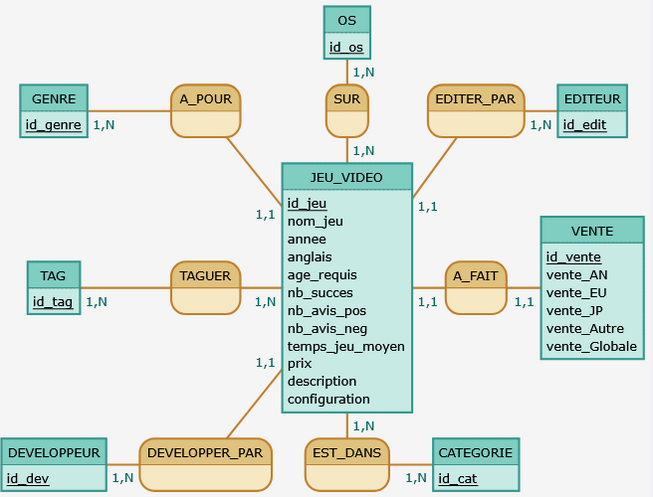
\includegraphics[width=\textwidth]{img/MCD.png}
  \caption{MCD}\label{MCD}
  }
  \end{figure}
  

\hypertarget{concluBD}{%
\section{\textbf{Conclusions}}\label{concluBD}}

La mise en place de la base de données nous a pris une semaine. Les difficultés étaient surtout de nettoyer les noms des jeux vidéo. En effet, certains jeux ont plusieurs noms différents, sur un csv il va être détaillé alors que sur l’autre ce sera un acronyme par exemple.
\normalsize


%%%%%%%%%%%%%%%%%%%%%%%%%%%%%%%%%%%%%
%%%%%%%%%%%%%%%%%%%%%%%%%%%%%%%%%%%%%
\hypertarget{Analyse-exploratoire-des-données}{%
\chapter{\textbf{Analyse exploratoire des données}}\label{AnalyseExploratoireDesDonnées}}

\hypertarget{IntroductionAnalyseExploratoireDesDonnées}{%
\section{\textbf{Introduction}}\label{IntroAnalyseExploratoireDesDonnées}}

Nous avons effectué toutes les analyses univariées et bivariées possibles. Nous avons aussi réalisé des tests du khi2, d’ANOVA et de corrélation linéaire. Cependant tous les graphiques obtenus n’étant pas forcément pertinents nous avons choisi de ne vous présenter que les 8 graphiques ci-dessous.

\hypertarget{DistributionDesVentes}{%
\section{\textbf{Distribution des ventes}}\label{DistributionDesVentes}}

  \begin{figure}[H]
  \hypertarget{distributionVentes}{%
  \centering
  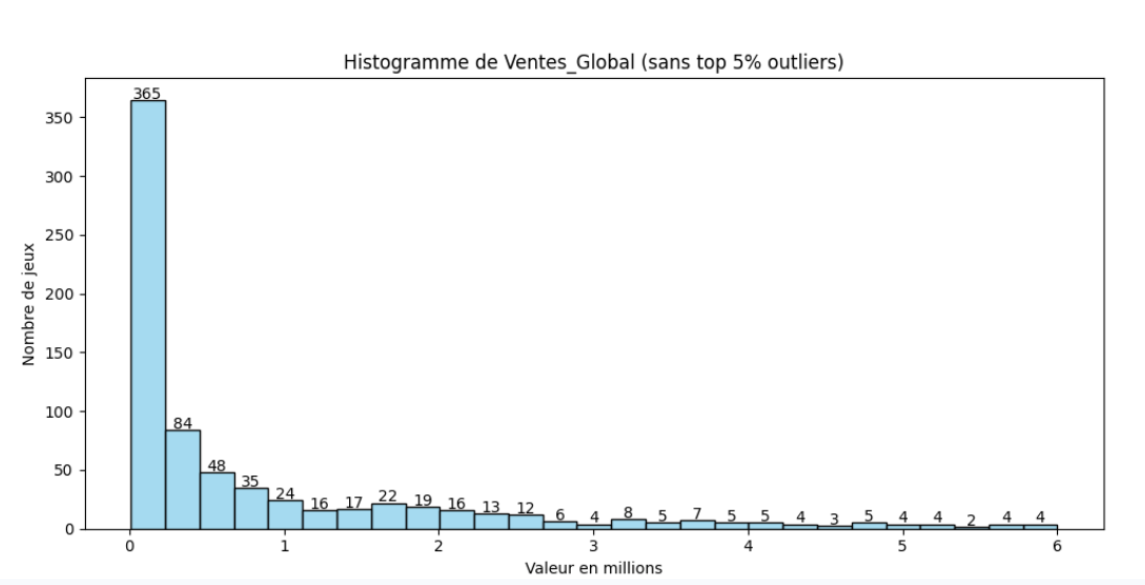
\includegraphics[width=\textwidth]{img/distributionVentes.png}
  \caption{Histogramme des ventes globales}\label{distributionVentes}
  }
  \end{figure}

Comme premier graphique à vous présenter, nous avons choisi cet histogramme. Il représente la relation entre le nombre de ventes et le nombre de jeux. Ici il est assez rapide de se rendre compte que la majeure partie des jeux présents constituant notre base de données ont été vendu en moins d’un million d’exemplaires (environ 70\%). Sur ce graphique nous avons aussi décidé de ne pas représenter les valeurs dites aberrantes afin d'améliorer la visibilité. Cette représentation de la dispersion de nos données nous a dès cet instant mis sur la route de proposer un modèle de prédiction qui s'orienterait vers des développeurs plutôt novices ou intermédiaires.

\hypertarget{CorrélationsEntreVariables}{%
\section{\textbf{Corrélations entre variables}}\label{CorrélationsEntreVariables}}

  \begin{figure}[H]
  \hypertarget{heatmap}{%
  \centering
  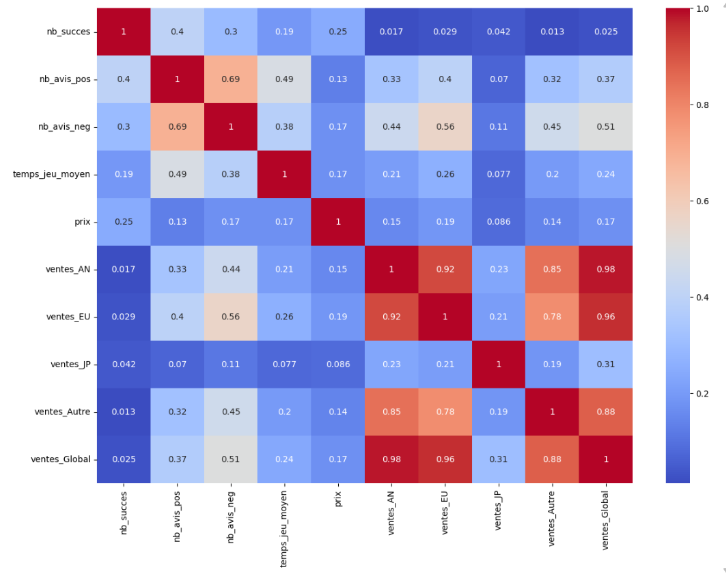
\includegraphics[width=\textwidth]{img/heatmap.png}
  \caption{Heatmap}\label{heatmap}
  }
  \end{figure}
  
Afin de mieux appréhender les graphes les plus importants à vous présenter, nous avons réalisé cette heatmap nous indiquant la corrélation entre les différentes variables. Plus les cases sont rouges, plus il existe une forte corrélation entre les variables. Une constatation intéressante et évidente concerne la corrélation entre les trois ``types'' de ventes entre Ventes\_AN, Ventes\_EU et Ventes\_Autre avec la variable Ventes\_globales. Cependant, l’indépendance de la variable Ventes\_JP avec ces autres variables est tout à fait inattendue. 

Mis à part ces constatations évidentes concernant les prix, il existe aussi une corrélation entre le nombre d’avis positifs et négatifs. De plus, nous pouvons aussi remarquer que la variable concernant le nombre d’avis négatifs a plus d’impact sur le nombre de ventes que la variable concernant le nombre d’avis positif. Cela peut refléter d’une certaine manière une tendance sociétale à faire davantage remarquer les points négatifs contrairement aux points positifs.


\hypertarget{RelationVentesEtAvis}{%
\section{\textbf{Relation ventes et avis}}\label{RelationVentesEtAvis}}

  \begin{figure}[H]
  \hypertarget{ventesAvis}{%
  \centering
  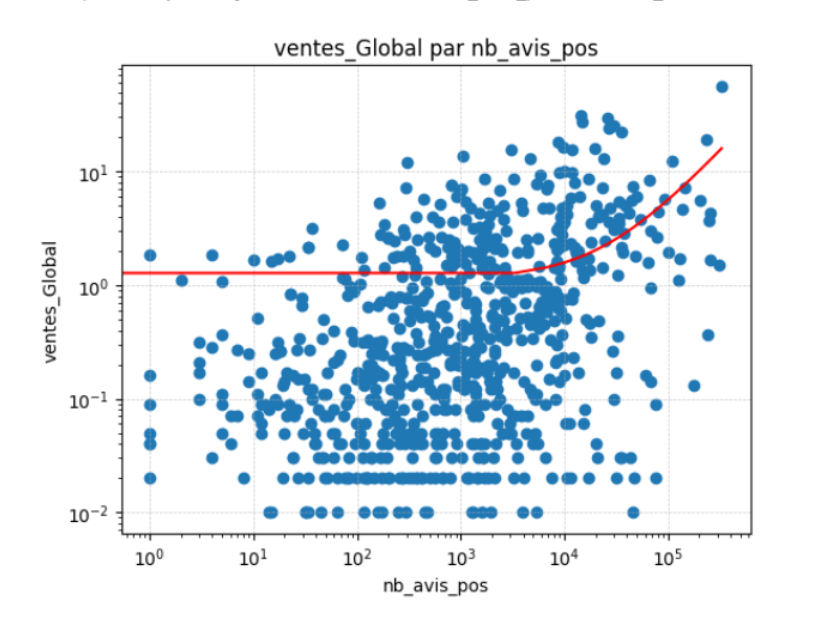
\includegraphics[width=\textwidth]{img/ventesAvis.png}
  \caption{Ventes globale par nombre d'avis possitif}\label{ventesAvis}
  }
  \end{figure}
  
  
Nous avons cependant tout de même décidé de vous montrer ce nuage de point (à l'échelle logarithmique) concernant la corrélation entre le nombre de ventes et le nombre d’avis positif. Nous avons, pour compléter ce graphique calculé le coefficient de corrélation qui nous indique que la droite obtenue explique seulement  13.39\% des données. De plus, nous avons calculé la p-value : avec 5\% de risques de se tromper , nous devons rejeter l’hypothèse induisant que les deux variables soient corrélées.

\hypertarget{AnalyseDesVentesParGenre}{%
\section{\textbf{Analyse des ventes par genre}}\label{AnalyseDesVentesParGenre}}

  \begin{figure}[H]
  \hypertarget{ventesGenre}{%
  \centering
  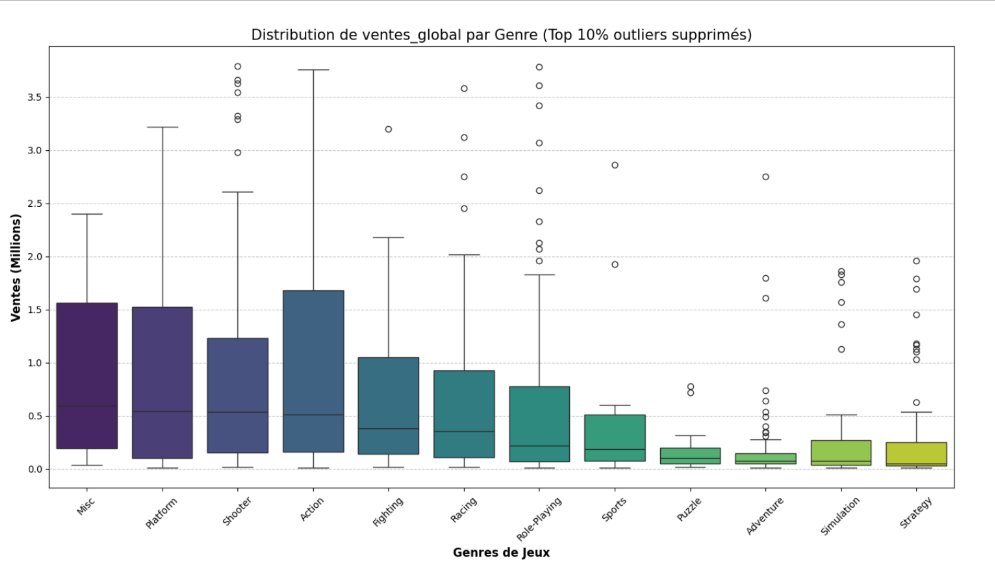
\includegraphics[width=\textwidth]{img/ventesGenre.png}
  \caption{Distribution des ventes globale par genre}\label{ventesGenre}
  }
  \end{figure}
  

Avec ces premiers box-plots représentant les ventes des jeux vidéo selon leur genre, nous pouvons très rapidement penser qu’il existe une corrélation entre ces deux variables. En effet, nous pouvons constater que les genres Puzzle, Adventure, Simulation, et Strategy sont moins vendus en un nombre d’exemplaire plus restreint. A contrario, les genres Action, Platform, Misc ont l’air de se vendre plus facilement, ou du moins en plus grand nombre. Il sera intéressant de comparer ces résultats avec le diagramme en mosaïque que l’on vous présentera plus tard et qui indiquera la proportion de jeux sortis par année selon leur genre.

\hypertarget{AnalyseDesVentesParAnnée}{%
\section{\textbf{Analyse des ventes par année}}\label{AnalyseDesVentesParAnnée}}

  \begin{figure}[H]
  \hypertarget{ventesAnnee}{%
  \centering
  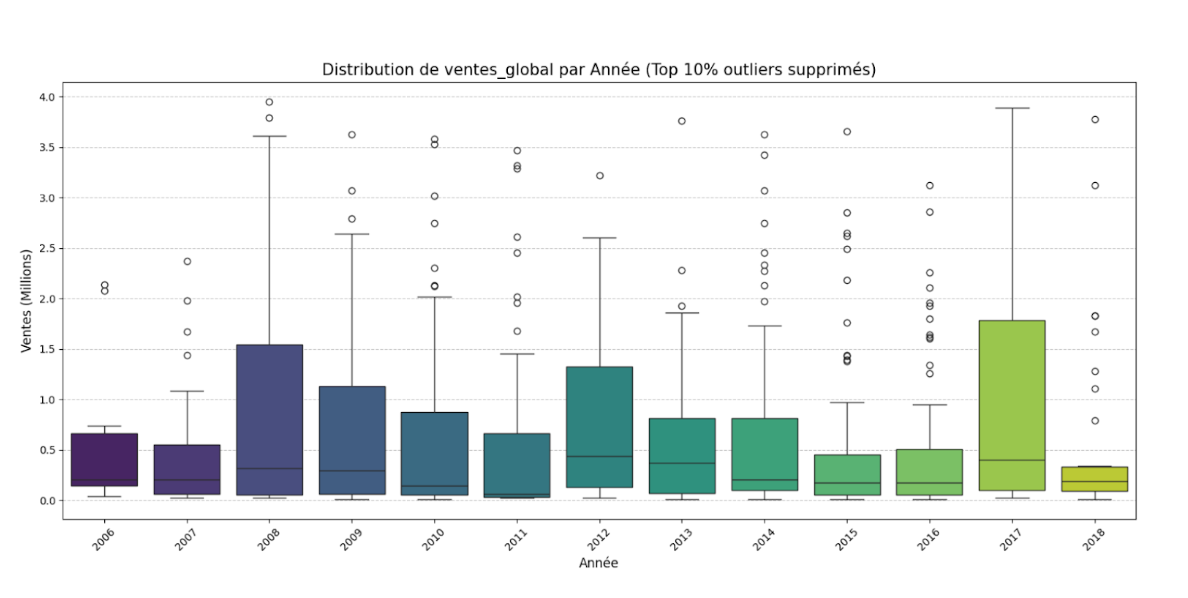
\includegraphics[width=\textwidth]{img/ventesAnnee.png}
  \caption{Distribution des ventes par année}\label{ventesAnnee}
  }
  \end{figure}
  
  
Par ce box-plot, nous souhaitions étudier la répartition des ventes des jeux vidéo suivant leur année de sortie. Tout d’abord nous savons ainsi que les jeux constituant notre base de données sont sortis entre 2008 et 2018. Ce graphique révèle une globale stabilité dans le nombre de ventes jusqu’en 2015. Cependant, durant l’année 2017 le nombre de ventes a fortement augmenté en devenant l’année avec le plus de ventes si l’on se base sur les quartiles et la médiane. En 2018, les données paraissent anormalement basses : c'est probablement dû au fait que nos données ne contiennent pas beaucoup de jeux sortis cette année-là, du à la suppression des valeurs aberrantes.

\hypertarget{RelationVentesEtPrixParPériode}{%
\section{\textbf{Relation ventes et prix par période}}\label{RelationVentesEtPrixParPériode}}

Ce graphique présente trois nuages de points illustrant la relation entre les ventes globales et les prix des jeux sortis, le tout divisé en trois périodes : 1998-2010, 2010-2015 et 2015-2020. Ce découpage a été fait afin de mieux observer l’évolution de cette relation au fil du temps.

Une première chose qui peut nous surprendre concerne la première période qui commence en 1998 pour se terminer en 2010. Si nous nous référons au graphe précédent, nos données ne débutent qu’à partir de 2008, cependant nous avions appliqué un filtre retirant les valeurs dites “aberrantes”. Cependant, concernant ce graphique qui sépare la nos données en 3 échelles de temps nous avons jugé préférable de garder toutes nos données. 


  \begin{figure}[H]
  \hypertarget{ventesPrix}{%
  \centering
  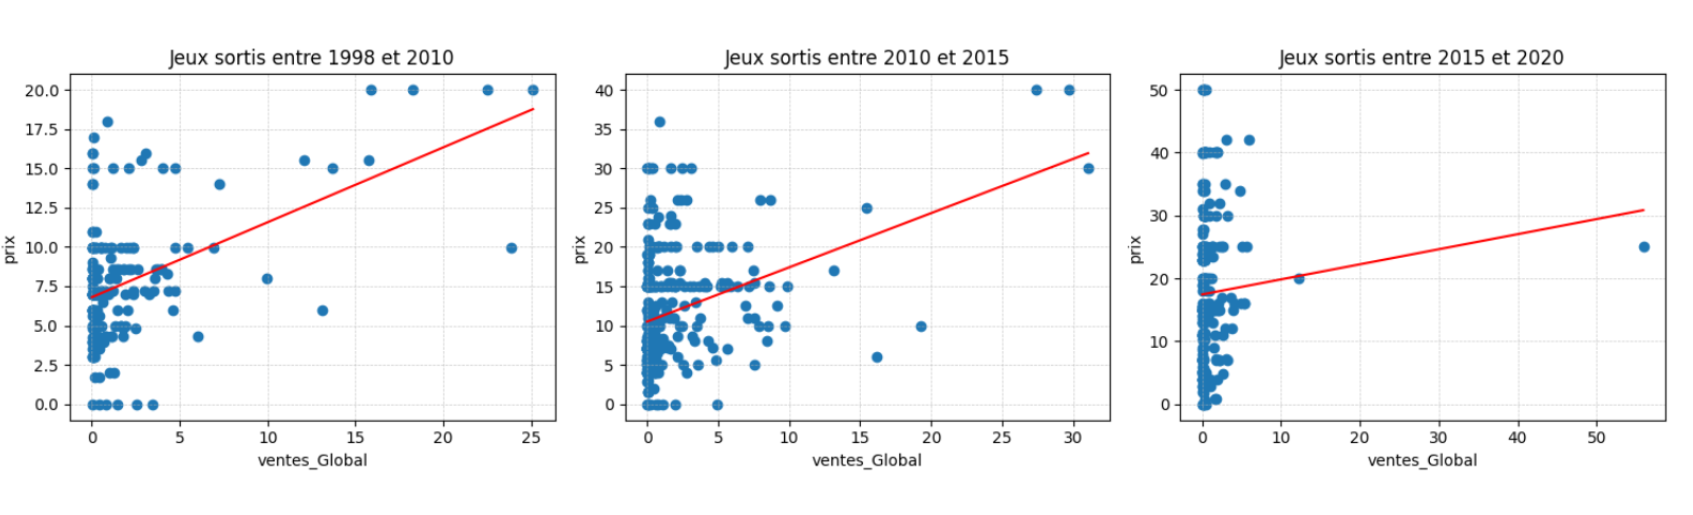
\includegraphics[width=\textwidth]{img/ventesPrix.png}
  \caption{Ventes globales par prix par période}\label{ventesPrix}
  }
  \end{figure}
  
  
A première vue, nos graphes semblent similaires. Cependant si nous prêtons attention aux échelles, nous pouvons très rapidement constater que la période 2010/2015 contient des jeux qui se sont vendus jusqu’à légèrement plus de 30 millions d’exemplaires et plus cher encore. Concernant la période 2015/2020, il y a moins de jeux qui se sont vendu en grand nombre d’exemplaires, cependant les jeux se vendent plus chers.

Cette fois-ci, pour garder une certaine cohérence, on a choisi de ne pas utiliser d’échelle logarithmique sur l’axe des abscisses. Sinon, ça aurait rendu la comparaison des graphes côte à côte plus compliquée et moins intuitive.

\hypertarget{ÉvolutionDesGenresDansLeTemps}{%
\section{\textbf{Évolution des genres dans le temps}}\label{ÉvolutionDesGenresDansLeTemps}}

  \begin{figure}[H]
  \hypertarget{mosaique}{%
  \centering
  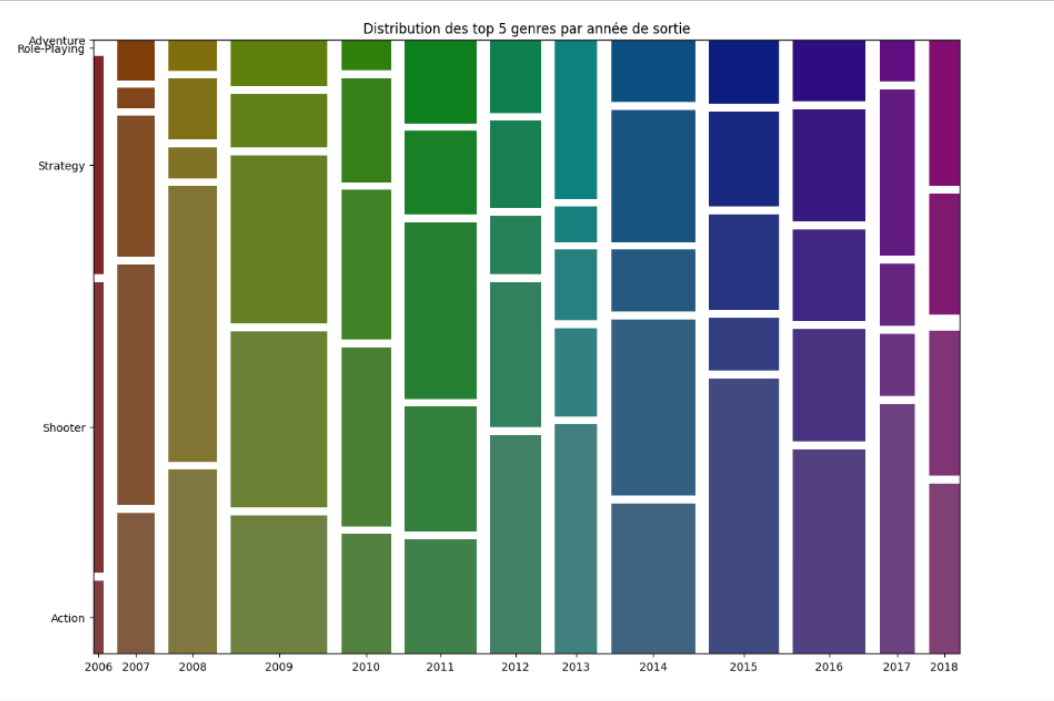
\includegraphics[width=\textwidth]{img/mosaique.png}
  \caption{Distribution des top 5 genres par année de sortie}\label{mosaique}
  }
  \end{figure}
  
Ce graphique mosaïque illustre l'évolution de la répartition des genres au fil des années. Nous constatons qu'entre 2006 et 2010, les jeux ``Shooter'' dominaient largement notre échantillon. Cependant, à partir de 2012, la catégorie ``Action'' prend la première place jusqu'à 2018. En parallèle, les autres genres comme la stratégie ou l'aventure fluctuent de manière beaucoup plus irrégulière selon les années. Ces variations prouvent que la structure du marché change selon l'époque. Il est donc nécessaire d'associer les variables genres et année pour que notre modèle intègre cette dimension temporelle dans ses prédictions.

\hypertarget{RépartitioDesCatégories}{%
\section{\textbf{Répartition des catégories}}\label{RépartitioDesCatégories}}

  \begin{figure}[H]
  \hypertarget{categories}{%
  \centering
  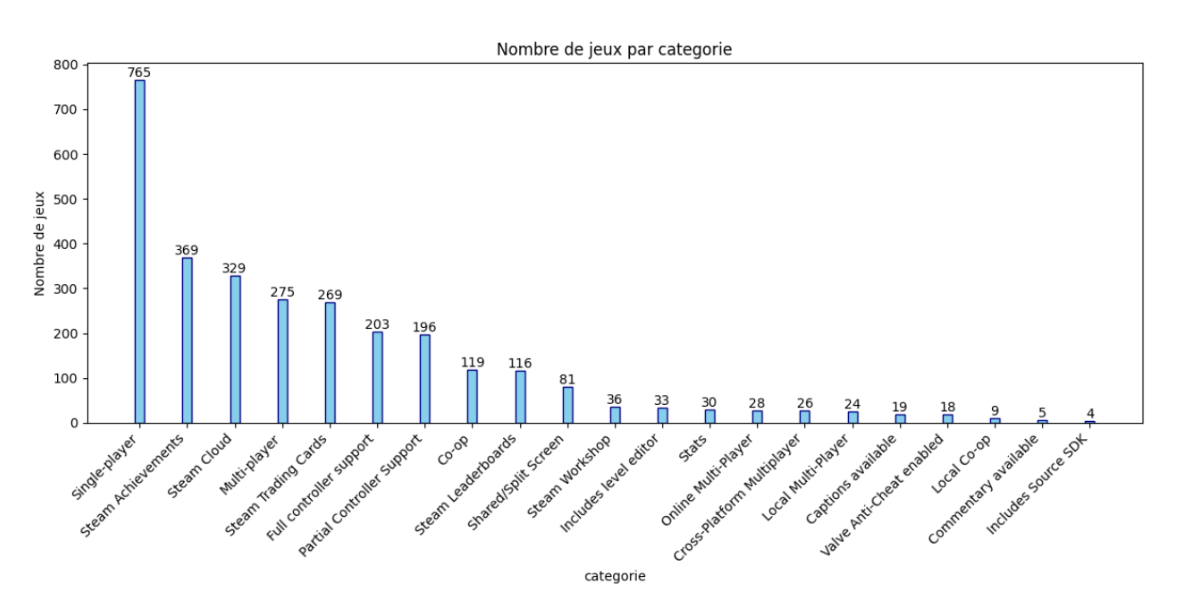
\includegraphics[width=\textwidth]{img/categories.png}
  \caption{nombre de jeux par categorie}\label{categories}
  }
  \end{figure}
  
Par la suite, nous avons réalisé ce diagramme afin de représenter la distribution des jeux selon les catégories auxquelles ils appartiennent. La première information évidente à retirer de ce graphique est la possibilité qu’un jeu appartienne à plusieurs catégories. Cela s’explique facilement avec le fait que beaucoup de jeux permettent à la fois de jouer en solitaire ou bien en équipe. Cependant, c'est bien la catégorie ``Single\_player'' qui regroupe le plus grand nombre de jeux (>95\%).

\hypertarget{AnalyseStatistiqueEtChoixMéthodologiques}{%
\section{\textbf{Analyse statistique et choix méthodologiques}}\label{AnalyseStatistiqueEtChoixMéthodologiques}}

Même si notre but est de prédire les ventes, tester les relations entre nos variables est une étape indispensable avant de les utiliser dans un modèle. Pour ce faire, nous nous sommes appuyées sur l'analyse de la variance (ANOVA), qui nous permet de voir comment les caractéristiques s'influencent mutuellement et de révéler des liens qui participent au succès d'un jeu.

En temps normal, on utilise la p-value pour évaluer si un effet est réel ou dû au hasard. Mais avec notre échantillon de 780 jeux, elle devient trop sensible : elle détecte comme significatives des différences si petites qu'elles n'ont en réalité aucun impact concret sur le modèle. Nous avons donc utilisé l'Eta-carré ($\eta^2$) à la place. Contrairement à la p-value qui nous dit seulement s'il y a un lien, l'Eta-carré mesure l'ampleur de ce lien en calculant le pourcentage de variation de notre cible expliqué par une variable. Savoir qu'un lien existe ne suffit pas, encore faut-il savoir s'il est assez puissant pour être utile.

Parmi les résultats les plus intéressants, on peut noter que la catégorie explique 87\% de la variance des avis négatifs ($\eta^2$ = 0.87), et qu'elle est également fortement liée aux ventes globales ($\eta^2$ = 0.668). Sachant que nous avions déjà constaté lors de notre analyse exploratoire que les avis négatifs impactent fortement les ventes, la catégorie apparaît donc comme un facteur particulièrement déterminant dans le succès d'un jeu, à la fois directement et via son influence sur les retours joueurs. À l'inverse, le système d'exploitation n'a pas d'effet significatif sur les ventes, que ce soit à l'échelle régionale ou mondiale (p-value > 0.14 et $\eta^2$ < 0.007). Cette analyse nous a permis de mieux comprendre le poids de chaque variable avant la modélisation, et de savoir quelles caractéristiques guideront réellement les prédictions de nos algorithmes.

%%%%%%%%%%%%%%%%%%%%%%%%%%%%%%%%%%%%%

\hypertarget{MachineLearning}{%
\chapter{\textbf{Machine Learning}}\label{MachineLearning}}

\hypertarget{ChoixDesVariablesExplicatives}{%
\section{\textbf{Choix des variables explicatives}}\label{ChoixDesVariablesExplicatives}}


Les 22 variables explicatives que nous avons sélectionnées peuvent être présentées sous forme de 4 familles : 

\begin{itemize}
\item Les caractéristiques du jeu avec : 
\begin{itemize}
\item L’âge requis : La tranche d’âge cible conditionne directement le public visé. Ainsi un jeu avec un âge minimum en seuil, le jeu exclut automatiquement une partie des acheteurs.
\item Le genre : c’est une des variables centrales. En effet, lors de nos analyses statistiques et représentations visuelles nous  avons représenté la distribution des ventes globales en fonction des genres, nous avons pu constater très rapidement que certains genres comme Action ou Platform génèrent beaucoup plus de ventes que Puzzle ou Strategy. 
\item Le prix : l’histogramme représentant les prix révèle une grande disparité de prix entre les jeux. De plus un autre graphe reliant le prix et le genre révèle aussi une forte variation dépendante du genre des jeux 
\item Le temps de jeu moyen : Le  box-plot représentant la distribution du temps de jeu moyen par genre, relate de façon évidente une corrélation faible mais stable  entre ces deux variables.
\item Le nombre de succès : Le graphe représentant le nombre de jeux par nombre de succès illustre la distribution de cette variable. Elle reflète la richesse du contenu d’un jeu.  
\end{itemize}

\item Les retours des joueurs avec :
\begin{itemize}
\item Les nombres d’avis positifs et négatifs: Le scatter plot représentant les nombres d’avis positifs avec les nombres d’avis négatifs montre une certaine corrélation entre ces deux variables. Après avoir réalisé un test du Khi2, au risque de 5\% nous pouvons affirmer que les deux variables sont corrélées. Ainsi nous aurions pu, ne mettre qu’une seule des deux variables dans le formulaire. En continuant les analyses nous avons pu constater que les avis négatifs avaient cependant plus d’impact sur le nombre de ventes que le nombre d’avis positifs. C’est pour cela que nous avons tout de même pris la décision de présenter les deux variables.
\item Les nombres de tags : la heatmap obtenue en reliant le genre avec les tags montre que les tags sont fortement liés aux autres caractéristiques du jeu. Ainsi, il était très important de la garder dans nos variables explicatives.
\end{itemize}

\item L’origine du jeu avec : 
\begin{itemize}
\item L’identifiant de l’éditeur : Le graphe représentant les 30 éditeurs qui ont eu en moyenne le plus grand nombre de ventes illustre à quel point les ventes peuvent varier selon les éditeurs. Par exemple, certains éditeurs comme Rockstar ou Activision ont des médianes sans commune mesure avec les autres. Cela justifie ainsi pleinement l’inclusion de cette variable.
\item L’identifiant du développeur :   le graphe représentant les 30 développeurs qui ont eu eux aussi en moyenne le plus grand nombre de ventes illustre lui aussi le même phénomène que le graphe concernant les éditeurs. Ainsi, les développeurs et éditeurs sont liés mais tout de même suffisamment distincts pour justifier la présence des deux variables.
\end{itemize}

\item Les caractéristiques techniques avec : 
\begin{itemize}
\item Les systèmes d’exploitation :  le graphique concernant la distribution des ventes global selon le système d’exploitation montre la différence certaine entre la popularité des systèmes d’exploitation. Cependant la heatmap concernant la distribution des OS par année de sortie révèle que la compatibilité évolue dans le temps. 
\item Les différentes catégories : solo, multi, online, vac, cloud, achiev, cards, ctrl, workshop sont représentées sur le graphique représentant la distribution de ventes globales par catégories. Ce graphique représente le nombre de ventes selon le jes modes disponibles. Ici encore nous pouvons constater que ces catégories ont un lien probables avec le nombre de ventes, c’est pourquoi nous avons décidé de les sélectionner afin d’affiner un maximum nos prédictions. 
\end{itemize}

\end{itemize}


\hypertarget{FiltrageDesDonnées}{%
\section{\textbf{Filtrage des données}}\label{FiltrageDesDonnées}}

En entraînant nos modèles, et en faisant l’analyse de nos données, nous nous sommes rendues compte que la majorité des jeux faisaient moins de 1M de ventes. Nous avons donc décidé de créer 3 types de modèles pour 3 types de jeux vidéo. On a fait une découpe ou l’on gardait tout le dataset sauf les ventes au dessus du 9ème décile que l’on nomme “dataset presque complet”, une autre où l’on gardait les jeux que l’on nomme “jeux moyens” (entre 270k et 3,8M de ventes), et enfin les jeux que l’on a nommé “petits jeux” qui font peu de ventes (dans la mesure des grands jeux vidéo), c’est à dire moins de 1,4M de ventes.

\hypertarget{ChoixDesModèlesDePrédiction}{%
\section{\textbf{Choix des modèles de prédiction}}\label{ChoixDesModèlesDePrédiction}}

Afin de mener à bien ce projet, il nous a fallu déterminer quels étaient les modèles de machine learning que nous souhaitions implémenter à l’intérieur. Pour cela nous nous sommes documentées longuement sur différents sites spécialisés dans le machine Learning. A la fin de nos recherches nous avons opté pour 3 modèles différents : Gradient Boosting, Random Forest, et Support Vector Regression. Pour des raisons pratiques nous n’avons finalement utilisé que les deux premiers modèles : Gradient Boosting et Random Forest. \\


\subsection{\textbf{Gradient Boosting}}

Le gradient boosting est une technique de machine learning qui combine plusieurs modèles de prédiction faibles pour former un seul ensemble. Ces modèles faibles sont généralement des arbres de décision, qui sont entraînés de manière séquentielle pour minimiser les erreurs et améliorer la précision. En combinant plusieurs arbres de régression ou de classification, le gradient boosting capte efficacement les relations complexes entre les caractéristiques. Un des principaux avantages de ce modèle est sa précision prédictive élevée. Cependant, il présente un inconvénient majeur : il est particulièrement exposé au surapprentissage, ce qui signifie que le modèle devient "trop adapté" aux données d'entraînement et perd sa capacité à généraliser. Pour y remédier, nos professeurs nous ont recommandé l'utilisation d'Optuna, un framework open-source d'optimisation automatique des hyperparamètres, que nous avons employé afin de déterminer les meilleures configurations pour tous nos modèles. Notre dataset contient 780 jeux et 22 variables de natures très différentes : des variables numériques continues (prix, temps de jeu moyen, nb d'avis), des variables binaires (os\_windows, os\_mac, cat\_solo, cat\_multi...) et des variables encodées (genre, éditeur, développeur). Le Gradient Boosting est particulièrement adapté à ce type de données hétérogènes car il est capable de capturer des interactions non linéaires complexes entre ces variables, comme par exemple l'effet combiné du prix et du genre sur les ventes.

Le Gradient Boosting repose sur plusieurs paramètres. Un premier paramètre est le n\_estimators, qui correspond au nombre d'arbres construits séquentiellement. Contrairement au Random Forest, ajouter trop d'arbres augmente ici le risque de surapprentissage. Le learning\_rate contrôle la contribution de chaque arbre au modèle final : un taux élevé apprend vite mais risque de rater le minimum optimal, un taux faible est plus prudent mais nécessite davantage d'arbres. Ces deux paramètres sont donc fortement liés et doivent être équilibrés ensemble. Le max\_depth limite la profondeur de chaque arbre : contrairement au Random Forest, les arbres du Gradient Boosting sont volontairement peu profonds car ils sont conçus pour corriger les erreurs progressivement plutôt que pour être précis individuellement. Le subsample définit la proportion des données utilisées pour entraîner chaque arbre : une valeur inférieure à 1 introduit de l'aléatoire, ce qui réduit le surapprentissage. Le min\_samples\_split et le min\_samples\_leaf fonctionnent de la même manière que pour le Random Forest : ils contrôlent la taille minimale des nœuds et des feuilles pour éviter des arbres trop spécifiques. Enfin, le max\_features détermine combien de features sont considérées à chaque division.

Nous avons mis dans notre fonction d'objectif pour Optuna des propositions à tester pour ces paramètres. Pour n\_estimators, nous avons proposé une plage allant de 50 à 500 par pas de 50. Pour le learning\_rate, nous avons appliqué une échelle logarithmique entre 0.01 et 0.3, afin qu'Optuna explore autant les petites valeurs que les grandes. Pour max\_depth, la plage est volontairement plus restreinte qu'en SVR, entre 2 et 8, car des arbres trop profonds en Gradient Boosting mènent rapidement au surapprentissage. Pour subsample, Optuna teste entre 0.5 et 1.0. Pour min\_samples\_split et min\_samples\_leaf, les plages vont respectivement de 2 à 20 et de 1 à 10. Enfin, pour max\_features, on lui a donné trois options : sqrt qui utilise la racine carrée du nombre de features, log2 qui utilise son logarithme en base 2, et None qui les utilise toutes. \\


\subsection{\textbf{Random Forest}}

Le Random Forest est un modèle de machine learning qui combine plusieurs arbres de décision, entraînés indépendamment sur des sous-échantillons aléatoires des données. Chaque arbre produit une prédiction, et le résultat final est obtenu en faisant la moyenne de toutes ces prédictions. En diversifiant ainsi les arbres, le Random Forest capture efficacement les relations complexes entre les caractéristiques tout en réduisant la variance. Un des principaux avantages de ce modèle est sa robustesse naturelle face au surapprentissage (contrairement à Gradient Boosting), grâce à la diversité des arbres qui le composent. Cependant, il peut manquer de précision sur certains datasets complexes par rapport à des méthodes séquentielles comme le Gradient Boosting. Pour optimiser ses performances, nous avons également utilisé Optuna afin de déterminer les meilleures configurations pour notre modèle Random Forest. Avec 22 variables dont une majorité de variables binaires (os, catégories), le Random Forest est particulièrement pertinent car il sélectionne aléatoirement un sous-ensemble de variables à chaque arbre, évitant ainsi que certaines variables très corrélées (comme cat\_solo et cat\_multi) ne dominent les prédictions. De plus, avec 780 observations, sa robustesse naturelle face au surapprentissage en fait un choix solide pour notre dataset de taille modérée.

Le Random Forest repose sur plusieurs paramètres. Un premier paramètre est le n\_estimators, qui correspond au nombre d'arbres dans la forêt. Plus il y en a, plus le modèle est stable, mais plus le temps de calcul augmente. Un deuxième paramètre est le max\_depth, qui limite la profondeur maximale de chaque arbre. Un arbre trop profond risque de mémoriser les données d'entraînement et de faire de l'overfitting. Le min\_samples\_split définit le nombre minimum d'échantillons nécessaires pour qu'un nœud se divise : une valeur élevée rend les arbres plus simples et donc plus généraux. Dans la même logique, le min\_samples\_leaf fixe le nombre minimum d'échantillons requis dans une feuille, ce qui empêche la création de branches trop spécifiques. Enfin, le max\_features détermine combien de features sont considérées à chaque division d'un nœud, ce qui introduit de l'aléatoire entre les arbres et favorise leur diversité.

Nous avons mis dans notre fonction d'objectif pour Optuna des propositions à tester pour ces paramètres. Pour n\_estimators, nous avons proposé une plage allant de 50 à 500 par pas de 50. Pour max\_depth, Optuna teste entre 2 et 20 niveaux de profondeur. Pour min\_samples\_split et min\_samples\_leaf, les plages vont respectivement de 2 à 20 et de 1 à 10. Enfin, pour max\_features, on lui a donné trois options : sqrt qui utilise la racine carrée du nombre de features, log2 qui utilise son logarithme en base 2, et None qui les utilise toutes. \\


\subsection{\textbf{Support Vector Regression}}

Le SVR ressemble à la régression linéaire, cependant, il en diffère puisqu’il cherche un “tunnel” autour de la droite plus ou moins large, appelé epsilon. Les points qui seront dans ce tunnel seront considérés comme “bien prédits” et seront donc ignorés. Pour construire le modèle, seulement les points en dehors de ce tunnel comptent. Un deuxième paramètre du SVR est le C. Le C contrôle la tolérance aux erreurs. En effet, un C élevé essaie de faire entrer un maximum de points dans le tunnel, ce qui peut créer de l’overfitting si trop élevé, et un C faible accepte plus d’erreurs. Nous pouvions rentrer d’autres paramètres dans nos fonctions, telles que le kernel. Le kernel sert à projeter les données dans un espace de dimension supérieure pour voir si les données deviennent linéaires, comme ça il peut faire la régression puis revenir dans l’espace original. Nous avions un dernier paramètre, le gamma. Le gamma contrôle à quelle vitesse l’influence d’un point diminue avec la distance. Avec un gamma élevé, chaque point n’influence que ses proches voisins, si trop élevé, il y a un risque d’overfitting. Avec un gamma faible, chaque point influence un voisinage plus large, ce qui rend le modèle plus général.

Nous avons mis dans notre fonction d’objectif pour Optuna des propositions à tester pour les paramètres. Pour C, nous avons proposé une plage allant de 0.1 à 100 avec une échelle logarithmique. Cette échelle permet d’éviter que Optuna passe trop de temps à tester des valeurs entre 50 et 100 par exemple et d’ignorer les petites valeurs. Pour epsilon, nous avons appliqué un logarithme également, entre 0.01 et 1. Pour le kernel, on laisse le choix à Optuna entre trois familles de modèles différents : rbf, linear, ou poly. Linear c’est le linéaire qui trace une droite, polynomial va tracer une courbe grâce à un polynôme, et rbf trace une courbe qui peut prendre n’importe quelle forme, c’est le plus flexible. Enfin, pour le gamma, on lui a donné 2 stratégies différentes à tester : scale ou auto. Scale tient en compte la dispersion des données alors que auto non.

Malgré ce que nous avions préparé, le SVR a une complexité quadratique qui a été incompatible avec la puissance de nos ordinateurs. En effet, le tuning avec Optuna prenait beaucoup trop de temps (plus de 20mins), nous avons donc décidé de ne pas utiliser ce modèle, mais de le laisser en commentaire dans le rapport au début pour que vous voyiez ce que nous avons fait. \\

	
\hypertarget{LesMétriquesUtilisées}{%
\section{\textbf{Les Métriques utilisées}}\label{LesMétriquesUtilisées}}

Le RMSE (Root Mean Squared Error) est la racine carrée de la moyenne des erreurs, le tout au carré. Elle pénalise fortement les grandes erreurs de prédiction. 

La MAE (Mean Absolute Error) est la moyenne des valeurs absolues des erreurs. Elle indique en moyenne de combien d'unités de ventes le modèle se trompe. Contrairement au RMSE, elle ne pénalise pas excessivement les grandes erreurs. Afin d’analyser le RMSE ou le MAE, il faut les rapporter à nos valeurs puisque ces erreurs sont exprimées dans l’unité de nos valeurs. Il faut aussi les analyser en fonction de notre contexte. Par exemple, un RMSE de 100 pourrait paraître grand, alors que si nos valeurs vont jusqu’à 1M, c’est en réalité petit, et d’un autre côté, une erreur de 1 suivant le contexte peut être énorme (par exemple dans un contexte de température corporelle).

Le R\textsuperscript{2} (Coefficient de Détermination) mesure la proportion de la variance des ventes expliquée par notre modèle. Sa valeur est comprise entre 0 et 1. Plus il est proche de 1, mieux le modèle explique les variations de ventes entre les jeux. Un R\textsuperscript{2} de 0.8 par exemple signifie que notre modèle explique 80\% des variations de ventes observées.

Ces trois métriques sont complémentaires et permettent d'avoir une vision complète et globale des performances de nos modèles. Le RMSE et le MAE mesurent toutes les deux les erreurs de prédiction en unités de ventes, mais de manière différente avec chacunes leurs points forts : le RMSE est plus sensible aux grandes erreurs ponctuelles, tandis que le MAE donne une vision plus globale et stable de l'erreur moyenne. Le R\textsuperscript{2} quand à lui apporte une perspective différente en indiquant la mesure dans laquelle notre modèle explique les variations de ventes entre les jeux.


\hypertarget{ChoixDeLalgorithmeDévaluationDeModèles}{%
\section{\textbf{Choix de l’algorithme d’évaluation de modèles}}\label{ChoixDeLalgorithmeDévaluationDeModèles}}

Après avoir discuté avec nos professeurs concernant la validation croisée avec la taille de notre dataset, ceux-ci nous ont conseillé d’utiliser l’algorithme Leave One and Out Cross Validation. Cet algorithme est très utile lorsque nous souhaitons utiliser l’ensemble de nos données à la fois pour l'entraînement de nos modèles, mais aussi pour les tests.

“\emph{La validation croisée est une méthode statistique d'évaluation des modèles qui consiste à partitionner les données en sous-ensembles pour l'entraînement et les tests. Au lieu d'une seule division en ensembles d'entraînement et de test, elle effectue plusieurs itérations de validation en utilisant différentes portions des données. 
[...]
Cette technique est précieuse lorsque les données sont limitées car elle maximise l'utilisation des données disponibles tout en fournissant des estimations fiables.}” (\href{https://medium.com/@pacosun/one-out-all-in-leave-one-out-cross-validation-explained-409df5ff6385}{medium.com})

Concernant Leave One and Out, chaque observation est utilisée à la fois pour l'entraînement du modèle, et à la fois comme test. Voici une représentation du déroulement d’un algorithme LOOCV. Nous constatons que cet algorithme est basé sur une boucle qui va tester tour à tour chaque donnée de façon indépendante en s’appuyant sur toutes les autres. C’est ainsi que chaque donnée sert à la fois comme donnée d'entraînement et comme donnée de test.


  \begin{figure}[H]
  \hypertarget{loocv}{%
  \centering
  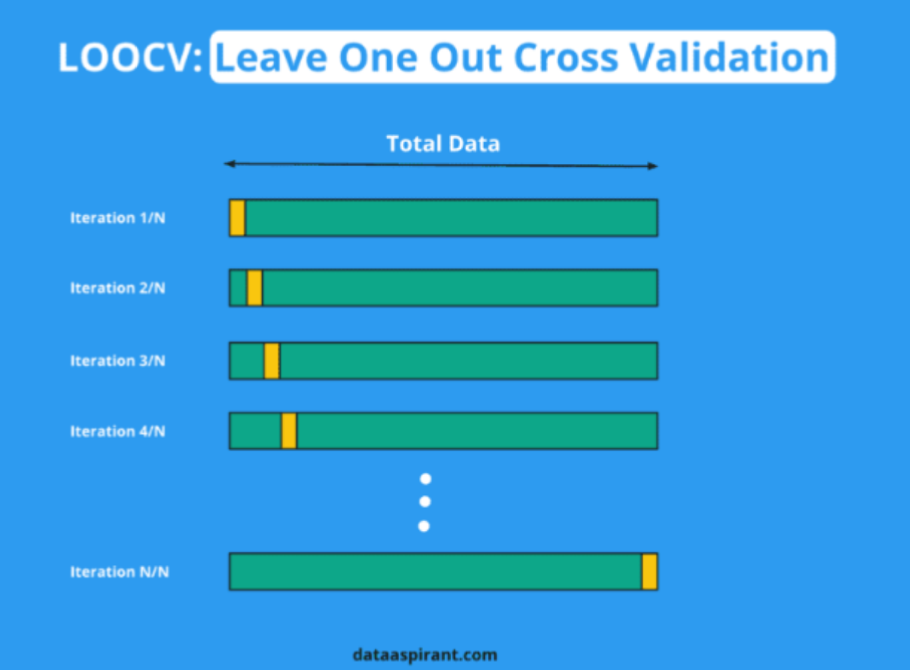
\includegraphics[height=7cm]{img/loocv.png}
  \caption{Leave One and Out Cross Validation}\label{loocv}
  }
  \end{figure}
  
  
Source : \href{https://medium.com/@pacosun/one-out-all-in-leave-one-out-cross-validation-explained-409df5ff6385}{dataaspirant}

Nos professeurs nous ont conseillés ce modèle d’algorithme en raison du petit nombre de données que nous possédons (<800). Nous sommes donc dans le cas où il est recommandé d’utiliser cet algorithme car au-delà de 1000 données la proportion entre la complexité temporelle et les résultats ne devient plus intéressante. Ainsi pour les jeux inférieurs à 1000 données c’est un des meilleurs algorithmes puisque chaque donnée est doublement utilisée

\hypertarget{ConclusionMachineLearning}{%
\section{\textbf{Conclusion Machine Learning}}\label{ConclusionMachineLearning}}

Au total, nous avons évalué 6 modèles via LOOCV : Gradient Boosting et Random Forest, chacun entraîné sur trois découpages du dataset (dataset complet, jeux moyens, petits jeux).

Sur le dataset presque complet, le Gradient Boosting ressort légèrement meilleur sur toutes les métriques (RMSE = 0.755M, MAE = 0.546M, R\textsuperscript{2} = 0.248), contre Random Forest (RMSE = 0.757M, MAE = 0.547M, R\textsuperscript{2} = 0.245). Les deux modèles sont cependant extrêmement proches. Concernant l'importance des variables, les deux modèles s'accordent sur des résultats similaires : nb\_tags, nb\_avis\_pos et nb\_avis\_neg dominent nettement, suivies par id\_developpeur, temps\_jeu\_moyen, id\_editeur et prix, avec des scores d'importance compris entre 0.06 et 0.1.

Sur les jeux moyens, les rôles s'inversent : Random Forest prend l'avantage sur le RMSE (0.830M contre 0.839M) et le R\textsuperscript{2} (0.207 contre 0.191), même si Gradient Boosting conserve un léger avantage sur la MAE (0.661M contre 0.668M). On remarque surtout une dégradation globale des performances pour les deux modèles sur ce découpage, ce qui en fait le moins fiable des trois. L'importance des variables évolue légèrement : nb\_tags reste en tête mais id\_developpeur monte en importance, ce qui suggère que pour les jeux moyens, l'identité du studio compte davantage.

Sur les petits jeux, Gradient Boosting reprend la tête sur toutes les métriques (RMSE = 0.228M, MAE = 0.171M, R\textsuperscript{2} = 0.180) contre Random Forest (RMSE = 0.231M, MAE = 0.175M, R\textsuperscript{2} = 0.153). Les valeurs de RMSE et MAE sont nettement plus faibles ici, ce qui s'explique logiquement par la plage de ventes bien plus réduite sur ce sous-dataset. On observe également un changement notable dans l'importance des variables : age\_requis et genre\_enc deviennent beaucoup plus déterminants (age\_requis représente à lui seul environ 35\% de l'importance dans Random Forest), tandis que nb\_tags recule significativement. Cela indique que sur ce segment, les caractéristiques intrinsèques du jeu pèsent plus que son exposition communautaire.

En conclusion, le Gradient Boosting est globalement le meilleur modèle, dominant sur 2 découpages sur 3 et sur la quasi-totalité des métriques. Les découpages dataset complet et petits jeux donnent par ailleurs les résultats les plus satisfaisants, tandis que le découpage jeux moyens peine à capturer la variance de cette tranche intermédiaire. Enfin, quelle que soit la configuration, les variables liées aux retours joueurs (avis positifs et négatifs) et au nombre de tags ressortent comme les plus importantes, confirmant a posteriori leur pertinence dans notre sélection initiale. Les performances restent cependant modestes sur l'ensemble des configurations (aucun modèle ne dépasse un R\textsuperscript{2} de 0.25) ce qui confirme que nos variables, bien que pertinentes, ne suffisent pas à capturer tous les facteurs qui font le succès commercial d'un jeu.


%%%%%%%%%%%%%%%%%%%%%%%%%%%%%%%%%%%%%

\hypertarget{LeSiteWeb}{%
\chapter{\textbf{Le site web}}\label{LeSiteWeb}}

\hypertarget{introSiteWeb}{%
\section{\textbf{Introduction}}\label{introSiteWeb}}

La création du site web permet à des développeurs d’estimer le nombre de ventes de leur jeu vidéo de manière simple et rapide. Il suffit de rentrer les informations demandées sur son jeu vidéo, de choisir un modèle de prédiction, et de cliquer sur un bouton. Afin d’accéder à notre site, voici le lien vers celui-ci : \texttt{https://gamessales.infinityfreeapp.com/}.

La création et la mise en place de l'API Flask et du site web se sont faites simultanément, comme vous le verrez décrit dans cette partie. Dans cette dernière, nous vous ferons tout d’abord une description technique de la mise en place des API, du site en lui-même avec sa structure, suivi d’une construction fonctionnelle du site.


\hypertarget{DescriptionTechnique}{%
\section{\textbf{Description technique}}\label{DescriptionTechnique}}

\subsection{\textbf{Création de l'API}}

Concernant l'API, nous avons tout d'abord créé un script Python à partir de notre fichier Jupyter traitant des modèles, dans lequel nous avons défini des fonctions pour charger les données et les prétraiter selon les trois profils décidés. Le but était de sauvegarder les modèles entraînés sous forme de fichiers “.pkl” pour éviter de les entraîner à chaque fois. C’est la bibliothèque Joblib qui a été utilisée à la fois pour créer ces fichiers et pour les charger.

L'API a été développée avec Flask, un Framework Python qui est utilisé pour créer l’API pour des sites web. Ce choix a été fait car Flask est simple à mettre en place et suffisant pour un projet de petite taille comme le nôtre. Le fichier “app.py” est le fichier principal : c’est lui qui gère les requêtes et les prédictions. Il charge les modèles ".pkl", associe le bon encodage à la variables “genre”, reçoit les données du formulaire au format JSON, les valide, les transmet au bon modèle, c’est-à-dire au modèle correspondant au profil de l'utilisateur, et retourne le résultat de la prédiction. Flask-CORS a également été ajouté pour autoriser les requêtes provenant du site web hébergé sur un domaine différent de celui de l'API. Sans lui, on avait des erreurs de blocage entre le site et l’API.

L'API a été déployée sur Render, qui propose une version gratuite suffisante pour notre projet, et se connecte directement à un dépôt GitHub pour redéployer automatiquement à chaque mise à jour du code. Le fichier “requirements.txt” liste toutes les bibliothèques Python nécessaires au fonctionnement de l'API comme Flask, scikit-learn ou joblib pour que Render puisse les installer automatiquement sans créer d’erreurs.


\subsection{\textbf{Structure du site}}

Avant de commencer la phase de codage du site web, nous avons créé plusieurs modules pour une meilleure organisation des fichiers. Regardons la structure de notre site web :

  \begin{figure}[H]
  \hypertarget{orgaSite}{%
  \centering
  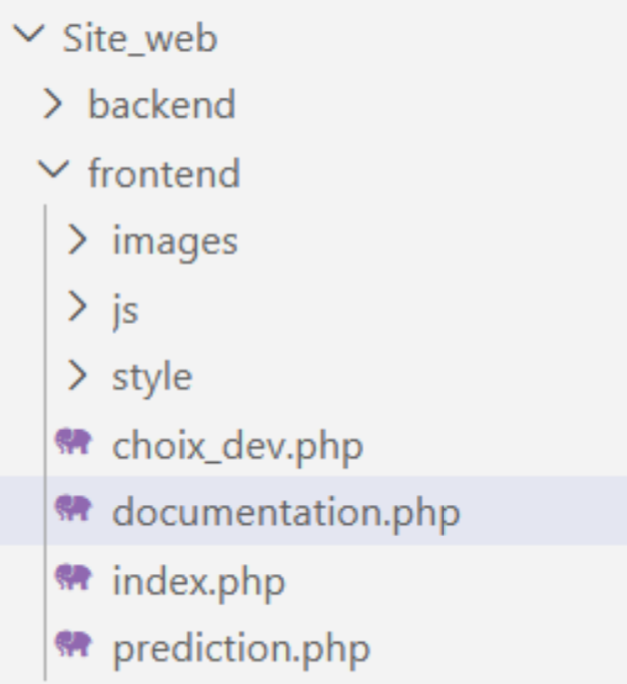
\includegraphics[height=7cm]{img/orgaSite.png}
  \caption{Structure du site}\label{orgaSite}
  }
  \end{figure}


Le dossier Site\_Web contient tous les fichiers du site. On y retrouve deux sous-dossiers principaux : backend et frontend. Comme vu tout à l’heure, le dossier backend regroupe tous les fichiers essentiels pour le bon fonctionnement de notre API, et donc de notre site. Le dossier frontend, quant à lui, contient tout ce qui concerne l’affichage et les interactions côté utilisateur : mise en page, formulaires et affichage des données. 

Le site web a été hébergé sur InfinityFree, un hébergeur gratuit choisi pour sa simplicité de prise en main et sa compatibilité avec notre stack technique et pour sa gratuité.


\hypertarget{Description fonctionnelle}{%
\section{\textbf{Description fonctionnelle}}\label{DescriptionF}}

\subsection{\textbf{Utilisateurs et conception}}


Tout d’abord, nous nous sommes questionnées sur l’identité de nos utilisateurs. On a utilisé nos compétences acquises lors du semestre 5 dans le module TE5PR1MI - Gestion de projet pour déterminer les différents types d’utilisateurs et leurs besoins. On en est arrivé à la réflexion suivante : le site s'adresse principalement aux développeurs de jeux vidéo, qu’ils soient peu connus ou relativement connus souhaitant obtenir une estimation, même approximative, concernant le nombre de ventes d'un de leurs jeux vidéo futurs ou en cours de développement ou de sortie.

Pour mieux savoir vers où nous diriger et par quels moyens, nous avons décidé de créer un Figma dans lequel seraient présentes les pages de notre site les plus importantes. C’est par contrainte de temps que nous avons choisi de faire seulement les pages les plus importantes et surtout de façon brève, c’est-à-dire qu’aucune des pages faite sur Figma n’étaient réellement terminées. Cependant, cela nous était amplement suffisant pour arriver à nous mettre d’accord sur la forme globale de notre site web.


\subsection{\textbf{Fonctionnement du site par écran}}

Écran 1 : Page de contextualisation

La première page de notre site est une page de contextualisation et de présentation. Cette page nous mène ensuite vers la page de choix du type de développeur.

Écran 2 : Choix du type de développeur

Cette page propose de sélectionner le niveau du développeur du jeu qu’on cherche à estimer : “petite” ou “toutes catégories de développeurs”. C’est ce choix qui va mener à un certain type de modèle de prédiction vu précédemment. Le choix du “petit développeur” ramène sur les modèles entraînés sur les données inférieures au 7ème décile et le choix du “toutes catégories de développeurs” utilise les modèles entraînés sur les données inférieures au 9ème décile. Ce découpage permet d’avoir des modèles plus adaptés selon le type de développeur. Une fois le choix du développeur fait, l’utilisateur est redirigé vers la page de prédiction. 


  \begin{figure}[H]
  \hypertarget{site1}{%
  \centering
  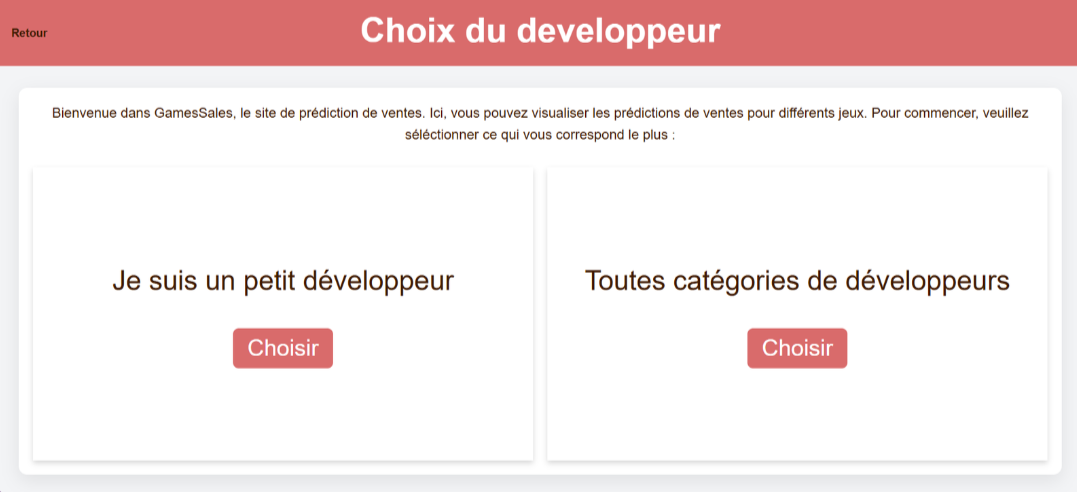
\includegraphics[width=\textwidth]{img/site1.png}
  \caption{Page de choix du développeur}\label{site1}
  }
  \end{figure}
  
  
Écran 3 : Page de prédiction

Depuis cette page de prédiction, l’utilisateur peut entrer ses données concernant le jeu qu’il souhaite estimer. Il doit alors remplir un formulaire de 22 questions. La grande majorité de ces questions concerne le jeu vidéo en lui-même. Tandis que d’autres peuvent être complété seulement une fois le jeu sortie au publique et avoir quelques retour : nombre d’avis positifs et nombre d’avis négatifs. Si le jeu n’est pas encore sorti ou s’il n’a pas encore de retour, il est possible de mettre la valeur “0”. Une fois tous les champs remplis, l’utilisateur à la possibilité de choisir le modèle avec lequel il souhaite faire des prédictions, Gradient Boosting ou Random Forest et lancer le programme d’approximation de ventes.

Pour rendre le site plus simple d’utilisation, des menus déroulants sont présents pour pratiquement tous les champs dans le but de montrer à l’utilisateur le type de réponse attendu pour ces questions. De plus, une sauvegarde des données saisis se fait automatiquement. Chaque modification est enregistrée pour que l’utilisateur puisse changer de catégorie de développeur et retrouver ses données sans avoir à les saisir à nouveau. Un bouton “Réinitialiser” à alors été ajouté pour pouvoir réinitialiser l'entièreté du formulaire. C’est une remise à zéro pour pouvoir remplir à nouveau tous les champs avec d’autres valeurs sans se perdre.


  \begin{figure}[H]
  \hypertarget{site2}{%
  \centering
  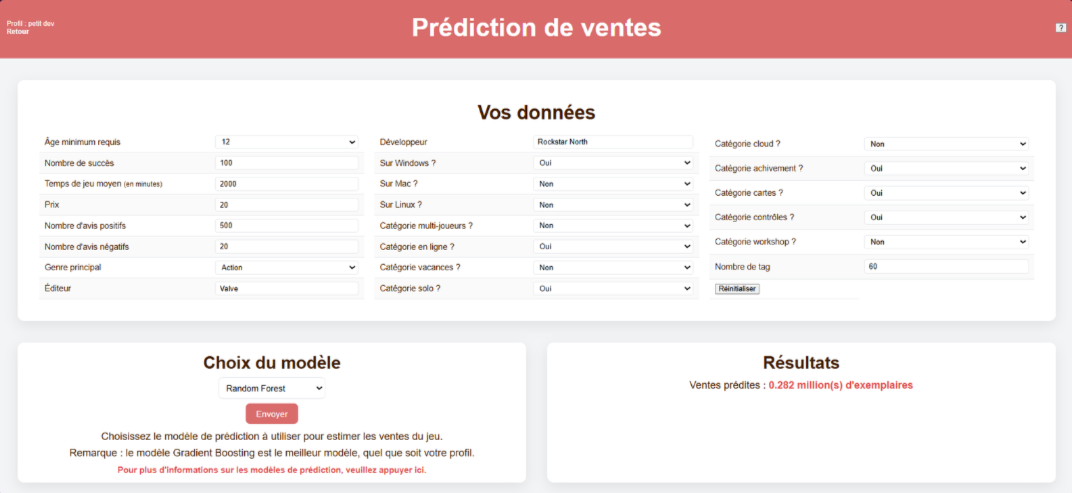
\includegraphics[width=\textwidth]{img/site2.png}
  \caption{Page de prédiction}\label{site2}
  }
  \end{figure}
  
  
Écran 4 : Page de documentation

Une page de documentation sur les modèles utilisés est accessible depuis la page de prédiction. Elle présente les résultats obtenus après évaluation de chaque modèle via le LOOCV (Leave-One-Out Cross Validation). On y retrouve les métriques d'évaluation RMSE, MAE et R\textsuperscript{2}, ainsi que les graphiques de comparaison entre les valeurs réelles et les valeurs prédites, pour chaque combinaison de modèle (Gradient Boosting, Random Forest) et de jeu de données (petit, grand). Une interprétation des métriques et une conclusion générale sont également présentes pour que l'utilisateur comprenne mieux les différences de performances de nos modèles.

  \begin{figure}[H]
  \hypertarget{site3}{%
  \centering
  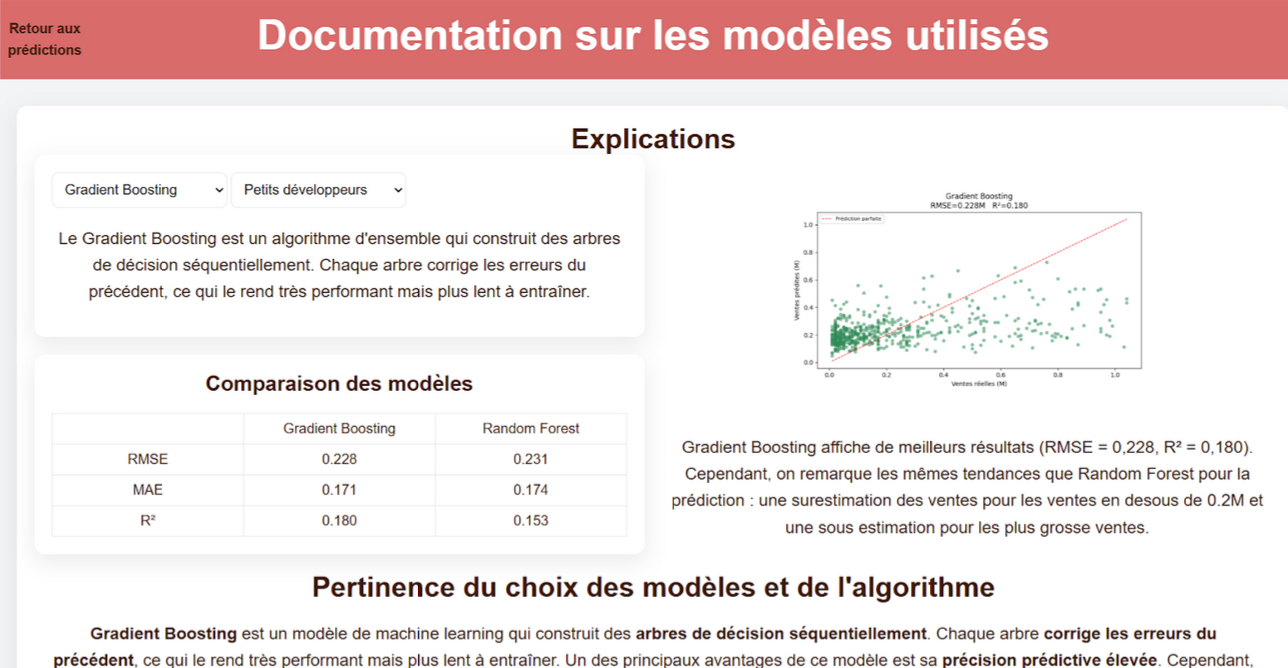
\includegraphics[width=\textwidth]{img/site3.png}
  \caption{Page documentation}\label{site3}
  }
  \end{figure}
  
  
\subsection{\textbf{Gestion des erreurs et sécurité}}


Plusieurs sécurités/restrictions ont été mises en place sur le site. Concernant les champs à valeurs numériques, l'utilisateur n’a pas le droit de saisir des valeurs négatives ni des décimales (seul le champ prix peut être un nombre à virgule mais doit rester positif). C’est pourquoi, une double sécurité a été implémentée : une première vérification côté client en HTML et en JavaScript qui bloque l'envoi du formulaire si une valeur invalide est détectée, et une seconde vérification côté serveur dans l'API Flask qui rejette la requête si les données reçues ne respectent pas les contraintes attendues. D'autres sécurités ont également été ajoutées : les champs binaires (Oui/Non) sont automatiquement forcés à 0 ou 1 côté client. Pour une meilleure expérience utilisateur, les champs Éditeur et Développeur disposent d'un système d'autocomplétion. Lorsque l'utilisateur commence à taper un nom, des suggestions apparaissent automatiquement. Ce système repose sur deux fichiers JSON générés au préalable depuis notre base de données (via un script Python écrit dans le fichier Machine Learning/export\_api/code\_json\_dev\_edit.py), contenant la correspondance entre les noms des éditeurs/développeurs et leurs identifiants internes. La traduction du nom vers identifiant se fait ensuite côté client en JavaScript. Si l'éditeur ou le développeur saisi n'est pas reconnu dans notre base, pas d’erreur affichée, la valeur “-1” est automatiquement envoyée à l'API, ce qui correspond à la valeur “inconnu” utilisée lors de l'entraînement des modèles.


%%%%%%%%%%%%%%%%%%%%%%%%%%%%%%%%%%%%%


\hypertarget{DifficultésRencontréesEtSolutionsApportées}{%
\section{\textbf{Difficultés rencontrées et solutions apportées}}\label{DifficultésRencontréesEtSolutionsApportées}}

Dans un premier temps, nous avions prévu d'utiliser une méthode classique de type train/test pour évaluer notre modèle de Machine Learning. Cependant, en nous interrogeant sur la pertinence de diviser un jeu de données déjà de petite taille en deux sous-ensembles distincts, nous avons réalisé que cette approche risquait de compromettre la fiabilité de nos résultats. Après en avoir discuté avec nos enseignants, ces derniers nous ont orientées vers la méthode Leave-One-Out (LOO), mieux adaptée aux petits jeux de données car elle maximise l'utilisation des données disponibles pour l'entraînement tout en permettant une évaluation rigoureuse du modèle. 

Ainsi, comme vous avez pu le voir précédemment dans notre rapport, nous vous avons présenté 2 modèles. Nous en avions pourtant retenu et codé un troisième : Support Vector Regression. Nous avons pris la décision de ne pas vous le présenter étant donné qu’il était trop long à s'exécuter. Nous avons donc été contraintes de renoncer à l’utiliser et ainsi nous limiter à seulement deux modèles. Cependant, nous avons tout de même laissé le code du modèle SVR dans le fichier Machine Learning présent dans l’espace de dépôt de notre Github.

Par la suite, après avoir mis en ligne notre site web sur l'hébergeur infinityfree, notre site web s’est retrouvé “suspendu”. Après nous être renseigné et avoir contacté nos enseignants, nous avons pu constater que l’option de l'hébergement gratuit du site impliquait des limites de temps d’accès. A partir de ce moment-là , nous avons réduit le nombre de connexions.

Un défi académique a été le décalage entre la date limite de rendu de la partie de Machine Learning et l'avancée de notre programme de Modélisation et Méthodes Statistiques. En effet, les concepts fondamentaux pour évaluer et ajuster des modèles de machine learning (la significance de MAE, RMSE et R²) ainsi que la théorie du sur-apprentissage (over-fitting) n'ont été abordés en cours qu'après notre deadline.

Un autre défi académique a été la nécessité de nous approprier par nous-mêmes certains concepts clés, tels que l'interprétation des métriques MAE, RMSE et R² ou la théorie du sur-apprentissage, qui n'avaient pas encore été abordés en cours au moment de la réalisation de cette partie du projet. Cela nous a amenées à effectuer un important travail de documentation personnelle en parallèle du développement des modèles.

Par ailleurs, l'analyse de notre jeu de données a mis en évidence une forte concentration des ventes autour de valeurs faibles : la majorité des jeux de notre base ont été vendus en moins d'un million d'exemplaires. Il aurait été intéressant de construire un modèle spécifiquement dédié à cette tranche de ventes, qui représente la réalité de la grande majorité des développeurs indépendants. Cependant, avec seulement 780 jeux au total, restreindre davantage le dataset aurait trop réduit la quantité de données disponibles pour l'entraînement, au risque de dégrader encore les performances des modèles.

Enfin, un problème en rapport avec Render est que nous l’avions relié au compte GitHub de Catherine, qui est la propriétaire/administrateur du projet GamesSales. Ainsi, à chaque nouveau push sur le dépôt de notre projet sur github, Render se met à jour automatiquement en utilisant la dernière version disponible du site. Cependant, elle seule avait accès au log, ce qui a compliqué les tests sur le site.

Ce projet a exigé de notre part un important travail de recherche en autonomie, car nous avons été confrontées à des concepts que nous n'avions encore jamais abordés. La construction et l'évaluation de nos algorithmes nécessitaient une compréhension de ces métriques spécifiques : (MAE, RMSE, R²); ainsi que la théorie du sur-apprentissage (over-fitting),. Toutes ces notions étaient certes au programme de notre semestre de troisième année, mais elles ne nous ont été expliquées en cours de modélisation qu’après la période où nous avons dû les mettre en pratique. Ainsi, nous avons complété nos connaissances par un grand travail personnel de documentation afin de mieux comprendre ce qu’il était attendu de nous.


%%%%%%%%%%%%%%%%%%%%%%%%%%%%%%%%%%%%%


\hypertarget{BilanDuProjetEtPerspectives}{%
\section{\textbf{Bilan du projet et perspectives}}\label{BilanDuProjetEtPerspectives}}

Au cours de ce projet, nous avons mené une démarche complète de data science : construction et nettoyage d'une base de données à partir de deux datasets Kaggle, analyse exploratoire approfondie, entraînement et évaluation de modèles de machine learning via LOOCV, et mise en ligne d'un site web fonctionnel permettant à des développeurs d'estimer les ventes de leur jeu. Nous avons entraîné 6 modèles au total (Gradient Boosting et Random Forest sur trois découpages du dataset), dont le meilleur atteint un R² de 0.248 sur le dataset complet.
Les performances restent modestes, ce qui s'explique principalement par la taille limitée du dataset (780 jeux) et par l'absence de variables explicatives clés. Cela ouvre cependant des pistes d'amélioration concrètes que nous détaillons ci-dessous.

Perspectives à court terme

La première amélioration prioritaire serait d'intégrer le modèle SVR, que nous avions entièrement codé et optimisé via Optuna mais que nous avons dû abandonner en raison de sa complexité quadratique, incompatible avec nos machines personnelles. Sur des machines plus puissantes (serveur de calcul ou cloud), son intégration complète (entraînement, évaluation LOOCV et ajout dans l'interface du site) représenterait environ 1 à 2 jours de travail. Cela permettrait d'avoir un troisième point de comparaison et potentiellement de meilleures prédictions sur certains découpages.

Une autre amélioration rapide concernerait l'infrastructure du site : partager les droits d'accès aux logs Render entre tous les membres du projet, et envisager une migration vers un hébergeur sans limite de connexions quotidiennes pour s'affranchir des contraintes d'InfinityFree.

Une autre piste d'amélioration à court terme concernerait la base de données elle-même. Par souci de simplicité et de temps, certains choix de modélisation ont été faits qui limitent aujourd'hui l'évolutivité de la base. Par exemple, la table genre n'a pas été conçue avec une table de jointure, partant du constat qu'un jeu n'appartient qu'à un seul genre dans notre dataset. Or, cette hypothèse simplificatrice pourrait ne pas tenir sur un dataset plus large ou plus récent. Revoir la structure de certaines tables pour les rendre plus flexibles et extensibles serait une étape importante avant d'envisager d'enrichir la base avec de nouvelles données.

Enfin, il serait pertinent de construire un modèle spécifiquement dédié aux jeux indépendants (moins de 1M de ventes), qui représentent la grande majorité des développeurs ciblés par notre outil. Ce modèle existe en partie dans notre découpage "petits jeux", mais il gagnerait à être entraîné sur un dataset plus fourni et mieux ciblé. Avec deux mois de travail, cela serait tout à fait faisable : scraping de données supplémentaires sur Steam, réentraînement des modèles et adaptation de l'interface du site pour guider l'utilisateur vers le bon modèle selon son profil.

Perspectives à long terme

Sur le plan de la data science, deux pistes nous semblent particulièrement prometteuses. La première serait d'exploiter les descriptions textuelles des jeux via du traitement du langage naturel (NLP). Nos descriptions sont actuellement inutilisées dans les modèles, alors qu'elles contiennent des informations qualitatives potentiellement riches : ton du jeu, univers, mécaniques mises en avant. Des techniques comme TF-IDF pourraient permettre d'en extraire des features supplémentaires et d'améliorer les prédictions.

La deuxième piste concerne l'enrichissement du dataset avec des variables marketing : budget publicitaire, présence sur les réseaux sociaux, couverture presse au moment de la sortie. Nos modèles n'expliquent actuellement qu'environ 20\% de la variance des ventes, ce qui suggère fortement que des facteurs externes au jeu lui-même jouent un rôle majeur. Ces données sont difficiles à obtenir automatiquement mais pourraient être collectées manuellement pour un sous-ensemble de jeux ou via des partenariats avec des acteurs du secteur.

Sur le plan métier, l'outil pourrait évoluer vers une plateforme de conseil plus complète pour les studios indépendants : non seulement estimer les ventes, mais aussi identifier quelles caractéristiques du jeu ont le plus d'impact sur ces estimations, et donc guider des décisions de développement (choix du genre, politique de prix, contenu communautaire).


%%%%%%%%%%%%%%%%%%%%%%%%%%%%%%%%%%%%%

\hypertarget{conclusion-et-perspectives}{%
\chapter{\textbf{Conclusions et perspectives}}\label{conclusion-et-perspectives}}


Ce projet nous a permis de mener une démarche complète de data science, de la construction d'une base de données à la mise en ligne d'un site web fonctionnel, en passant par l'analyse exploratoire et l'entraînement de modèles de machine learning. Travailler sur une thématique que nous connaissions déjà (les jeux vidéo) nous a permis de nous concentrer sur les aspects techniques et méthodologiques plutôt que sur la compréhension du domaine.

Nos résultats de prédiction restent modestes : avec un R² moyen d'environ 20\%, nos modèles n'expliquent qu'une faible part de la variance des ventes. Cette limitation s'explique principalement par la taille restreinte de notre dataset (780 jeux) et par l'absence de variables clés comme les budgets publicitaires ou la notoriété des studios. Malgré tout, le Gradient Boosting s'est révélé être notre meilleur modèle, et le site web permet d'en exploiter les prédictions de façon accessible et intuitive.

Sur le plan académique, ce projet nous a poussées à nous approprier par nous-mêmes des notions (validation croisée, métriques d'évaluation, surapprentissage) que nous découvrions souvent en parallèle de leur mise en pratique. C'est sans doute l'un des apprentissages les plus formateurs de ce semestre. Nous repartons avec une vision plus réaliste des contraintes d'un projet de bout en bout, et des pistes claires pour améliorer ce travail si l'occasion se représentait.


\end{document}

